\documentclass[twoside]{book}

% Packages required by doxygen
\usepackage{fixltx2e}
\usepackage{calc}
\usepackage{doxygen}
\usepackage[export]{adjustbox} % also loads graphicx
\usepackage{graphicx}
\usepackage[utf8]{inputenc}
\usepackage{makeidx}
\usepackage{multicol}
\usepackage{multirow}
\PassOptionsToPackage{warn}{textcomp}
\usepackage{textcomp}
\usepackage[nointegrals]{wasysym}
\usepackage[table]{xcolor}

% Font selection
\usepackage[T1]{fontenc}
\usepackage[scaled=.90]{helvet}
\usepackage{courier}
\usepackage{amssymb}
\usepackage{sectsty}
\renewcommand{\familydefault}{\sfdefault}
\allsectionsfont{%
  \fontseries{bc}\selectfont%
  \color{darkgray}%
}
\renewcommand{\DoxyLabelFont}{%
  \fontseries{bc}\selectfont%
  \color{darkgray}%
}
\newcommand{\+}{\discretionary{\mbox{\scriptsize$\hookleftarrow$}}{}{}}

% Page & text layout
\usepackage{geometry}
\geometry{%
  a4paper,%
  top=2.5cm,%
  bottom=2.5cm,%
  left=2.5cm,%
  right=2.5cm%
}
\tolerance=750
\hfuzz=15pt
\hbadness=750
\setlength{\emergencystretch}{15pt}
\setlength{\parindent}{0cm}
\setlength{\parskip}{3ex plus 2ex minus 2ex}
\makeatletter
\renewcommand{\paragraph}{%
  \@startsection{paragraph}{4}{0ex}{-1.0ex}{1.0ex}{%
    \normalfont\normalsize\bfseries\SS@parafont%
  }%
}
\renewcommand{\subparagraph}{%
  \@startsection{subparagraph}{5}{0ex}{-1.0ex}{1.0ex}{%
    \normalfont\normalsize\bfseries\SS@subparafont%
  }%
}
\makeatother

% Headers & footers
\usepackage{fancyhdr}
\pagestyle{fancyplain}
\fancyhead[LE]{\fancyplain{}{\bfseries\thepage}}
\fancyhead[CE]{\fancyplain{}{}}
\fancyhead[RE]{\fancyplain{}{\bfseries\leftmark}}
\fancyhead[LO]{\fancyplain{}{\bfseries\rightmark}}
\fancyhead[CO]{\fancyplain{}{}}
\fancyhead[RO]{\fancyplain{}{\bfseries\thepage}}
\fancyfoot[LE]{\fancyplain{}{}}
\fancyfoot[CE]{\fancyplain{}{}}
\fancyfoot[RE]{\fancyplain{}{\bfseries\scriptsize Generated by Doxygen }}
\fancyfoot[LO]{\fancyplain{}{\bfseries\scriptsize Generated by Doxygen }}
\fancyfoot[CO]{\fancyplain{}{}}
\fancyfoot[RO]{\fancyplain{}{}}
\renewcommand{\footrulewidth}{0.4pt}
\renewcommand{\chaptermark}[1]{%
  \markboth{#1}{}%
}
\renewcommand{\sectionmark}[1]{%
  \markright{\thesection\ #1}%
}

% Indices & bibliography
\usepackage{natbib}
\usepackage[titles]{tocloft}
\setcounter{tocdepth}{3}
\setcounter{secnumdepth}{5}
\makeindex

% Hyperlinks (required, but should be loaded last)
\usepackage{ifpdf}
\ifpdf
  \usepackage[pdftex,pagebackref=true]{hyperref}
\else
  \usepackage[ps2pdf,pagebackref=true]{hyperref}
\fi
\hypersetup{%
  colorlinks=true,%
  linkcolor=blue,%
  citecolor=blue,%
  unicode%
}

% Custom commands
\newcommand{\clearemptydoublepage}{%
  \newpage{\pagestyle{empty}\cleardoublepage}%
}

\usepackage{caption}
\captionsetup{labelsep=space,justification=centering,font={bf},singlelinecheck=off,skip=4pt,position=top}

%===== C O N T E N T S =====

\begin{document}

% Titlepage & ToC
\hypersetup{pageanchor=false,
             bookmarksnumbered=true,
             pdfencoding=unicode
            }
\pagenumbering{alph}
\begin{titlepage}
\vspace*{7cm}
\begin{center}%
{\Large Acoustic-\/\+M\+U\+S\+IC }\\
\vspace*{1cm}
{\large Generated by Doxygen 1.8.13}\\
\end{center}
\end{titlepage}
\clearemptydoublepage
\pagenumbering{roman}
\tableofcontents
\clearemptydoublepage
\pagenumbering{arabic}
\hypersetup{pageanchor=true}

%--- Begin generated contents ---
\chapter{File Index}
\section{File List}
Here is a list of all documented files with brief descriptions\+:\begin{DoxyCompactList}
\item\contentsline{section}{src/pinger\+\_\+localization/src/{\bfseries config.\+h} }{\pageref{pinger__localization_2src_2config_8h}}{}
\item\contentsline{section}{src/pinger\+\_\+localization/src/\hyperlink{main_8c}{main.\+c} \\*Runs M\+U\+S\+IC for an acoustic localization system }{\pageref{main_8c}}{}
\item\contentsline{section}{src/pinger\+\_\+localization/src/\hyperlink{matrix_8c}{matrix.\+c} \\*Functions used for real and complex matrix operations }{\pageref{matrix_8c}}{}
\item\contentsline{section}{src/pinger\+\_\+localization/src/\hyperlink{matrix_8h}{matrix.\+h} \\*Function declarations for real and complex matrix operations }{\pageref{matrix_8h}}{}
\item\contentsline{section}{src/pinger\+\_\+localization/src/\hyperlink{music_8c}{music.\+c} \\*Functions used to compute D\+OA (direction-\/of-\/arrival) using M\+U\+S\+IC }{\pageref{music_8c}}{}
\item\contentsline{section}{src/pinger\+\_\+localization/src/\hyperlink{music_8h}{music.\+h} \\*Function declarations for M\+U\+S\+IC (Multiple Signal Classification) }{\pageref{music_8h}}{}
\item\contentsline{section}{src/pinger\+\_\+simulation/src/{\bfseries config.\+h} }{\pageref{pinger__simulation_2src_2config_8h}}{}
\item\contentsline{section}{src/pinger\+\_\+simulation/src/\hyperlink{simulate_8c}{simulate.\+c} \\*Simulates sampling a pinger in an underwater environment }{\pageref{simulate_8c}}{}
\end{DoxyCompactList}

\chapter{File Documentation}
\hypertarget{pinger__localization_2src_2config_8h}{}\section{src/pinger\+\_\+localization/src/config.h File Reference}
\label{pinger__localization_2src_2config_8h}\index{src/pinger\+\_\+localization/src/config.\+h@{src/pinger\+\_\+localization/src/config.\+h}}


Contains constants needed to calculate D\+OA (direction-\/of-\/arrival).  


This graph shows which files directly or indirectly include this file\+:\nopagebreak
\begin{figure}[H]
\begin{center}
\leavevmode
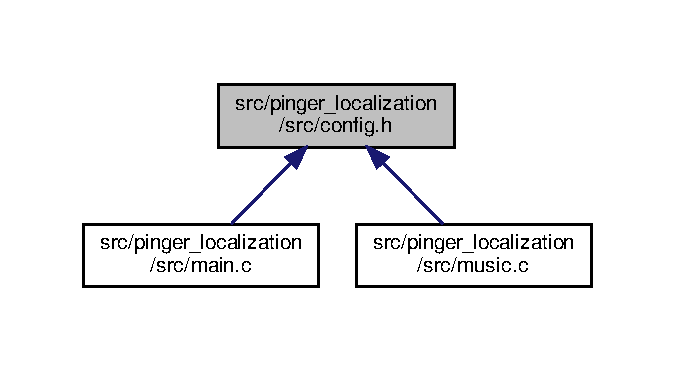
\includegraphics[width=324pt]{pinger__localization_2src_2config_8h__dep__incl}
\end{center}
\end{figure}
\subsection*{Variables}
\begin{DoxyCompactItemize}
\item 
const double \hyperlink{pinger__localization_2src_2config_8h_a9e8a46a0e00368ad98642587ca4ebdbe}{C} = 1480.
\item 
const double \hyperlink{pinger__localization_2src_2config_8h_a7a6b19aebea6b1104b347e66042a8817}{FS} = 400000.
\item 
const double \hyperlink{pinger__localization_2src_2config_8h_a5947531331b6f35777ca36c1077706b2}{F0} = 25000.
\item 
const double \hyperlink{pinger__localization_2src_2config_8h_aa5502bd8a25ebfb5c52692c708af2fe9}{S\+P\+A\+C\+I\+NG} = 0.\+0127
\item 
const double \hyperlink{pinger__localization_2src_2config_8h_acd7cffa257314a0c3ed206766758ddd9}{S\+E\+A\+R\+C\+H\+\_\+\+I\+N\+T\+E\+R\+V\+AL} = 0.\+1
\item 
const int \hyperlink{pinger__localization_2src_2config_8h_a2078d250ff41c35b39b40b9851765183}{N\+\_\+\+P\+HN} = 4
\item 
const int \hyperlink{pinger__localization_2src_2config_8h_ad72dfe6a84df9f192b62856b1cc697d0}{N\+\_\+\+D\+FT} = 2048
\item 
const int \hyperlink{pinger__localization_2src_2config_8h_ab2b6b0c222cd1ce70d6a831f57241e59}{N} = 16
\item 
const int \hyperlink{pinger__localization_2src_2config_8h_a9edc6895d567e0ddcdd3cc20df3f3b4b}{M} = 2
\item 
const int \hyperlink{pinger__localization_2src_2config_8h_afec54c0b8794d59c37e8b7822ff5e006}{D\+E\+B\+UG} = 0
\end{DoxyCompactItemize}


\subsection{Detailed Description}
Contains constants needed to calculate D\+OA (direction-\/of-\/arrival). 

These values should match the simulated settings in pinger\+\_\+simulation, or represent real world settings.

\begin{DoxyAuthor}{Author}
David Zhang (Davarco) 
\end{DoxyAuthor}


\subsection{Variable Documentation}
\mbox{\Hypertarget{pinger__localization_2src_2config_8h_a9e8a46a0e00368ad98642587ca4ebdbe}\label{pinger__localization_2src_2config_8h_a9e8a46a0e00368ad98642587ca4ebdbe}} 
\index{pinger\+\_\+localization/src/config.\+h@{pinger\+\_\+localization/src/config.\+h}!C@{C}}
\index{C@{C}!pinger\+\_\+localization/src/config.\+h@{pinger\+\_\+localization/src/config.\+h}}
\subsubsection{\texorpdfstring{C}{C}}
{\footnotesize\ttfamily const double C = 1480.}

Wave speed (m/s). \mbox{\Hypertarget{pinger__localization_2src_2config_8h_afec54c0b8794d59c37e8b7822ff5e006}\label{pinger__localization_2src_2config_8h_afec54c0b8794d59c37e8b7822ff5e006}} 
\index{pinger\+\_\+localization/src/config.\+h@{pinger\+\_\+localization/src/config.\+h}!D\+E\+B\+UG@{D\+E\+B\+UG}}
\index{D\+E\+B\+UG@{D\+E\+B\+UG}!pinger\+\_\+localization/src/config.\+h@{pinger\+\_\+localization/src/config.\+h}}
\subsubsection{\texorpdfstring{D\+E\+B\+UG}{DEBUG}}
{\footnotesize\ttfamily const int D\+E\+B\+UG = 0}

Log option. \mbox{\Hypertarget{pinger__localization_2src_2config_8h_a5947531331b6f35777ca36c1077706b2}\label{pinger__localization_2src_2config_8h_a5947531331b6f35777ca36c1077706b2}} 
\index{pinger\+\_\+localization/src/config.\+h@{pinger\+\_\+localization/src/config.\+h}!F0@{F0}}
\index{F0@{F0}!pinger\+\_\+localization/src/config.\+h@{pinger\+\_\+localization/src/config.\+h}}
\subsubsection{\texorpdfstring{F0}{F0}}
{\footnotesize\ttfamily const double F0 = 25000.}

Pinger frequency (Hz). \mbox{\Hypertarget{pinger__localization_2src_2config_8h_a7a6b19aebea6b1104b347e66042a8817}\label{pinger__localization_2src_2config_8h_a7a6b19aebea6b1104b347e66042a8817}} 
\index{pinger\+\_\+localization/src/config.\+h@{pinger\+\_\+localization/src/config.\+h}!FS@{FS}}
\index{FS@{FS}!pinger\+\_\+localization/src/config.\+h@{pinger\+\_\+localization/src/config.\+h}}
\subsubsection{\texorpdfstring{FS}{FS}}
{\footnotesize\ttfamily const double FS = 400000.}

Sampling speed (Hz). \mbox{\Hypertarget{pinger__localization_2src_2config_8h_a9edc6895d567e0ddcdd3cc20df3f3b4b}\label{pinger__localization_2src_2config_8h_a9edc6895d567e0ddcdd3cc20df3f3b4b}} 
\index{pinger\+\_\+localization/src/config.\+h@{pinger\+\_\+localization/src/config.\+h}!M@{M}}
\index{M@{M}!pinger\+\_\+localization/src/config.\+h@{pinger\+\_\+localization/src/config.\+h}}
\subsubsection{\texorpdfstring{M}{M}}
{\footnotesize\ttfamily const int M = 2}

Number of signal receivers per M\+U\+S\+IC calculation. \mbox{\Hypertarget{pinger__localization_2src_2config_8h_ab2b6b0c222cd1ce70d6a831f57241e59}\label{pinger__localization_2src_2config_8h_ab2b6b0c222cd1ce70d6a831f57241e59}} 
\index{pinger\+\_\+localization/src/config.\+h@{pinger\+\_\+localization/src/config.\+h}!N@{N}}
\index{N@{N}!pinger\+\_\+localization/src/config.\+h@{pinger\+\_\+localization/src/config.\+h}}
\subsubsection{\texorpdfstring{N}{N}}
{\footnotesize\ttfamily const int N = 16}

Number of points to simulate for signal. \mbox{\Hypertarget{pinger__localization_2src_2config_8h_ad72dfe6a84df9f192b62856b1cc697d0}\label{pinger__localization_2src_2config_8h_ad72dfe6a84df9f192b62856b1cc697d0}} 
\index{pinger\+\_\+localization/src/config.\+h@{pinger\+\_\+localization/src/config.\+h}!N\+\_\+\+D\+FT@{N\+\_\+\+D\+FT}}
\index{N\+\_\+\+D\+FT@{N\+\_\+\+D\+FT}!pinger\+\_\+localization/src/config.\+h@{pinger\+\_\+localization/src/config.\+h}}
\subsubsection{\texorpdfstring{N\+\_\+\+D\+FT}{N\_DFT}}
{\footnotesize\ttfamily const int N\+\_\+\+D\+FT = 2048}

Number of points in D\+FT. \mbox{\Hypertarget{pinger__localization_2src_2config_8h_a2078d250ff41c35b39b40b9851765183}\label{pinger__localization_2src_2config_8h_a2078d250ff41c35b39b40b9851765183}} 
\index{pinger\+\_\+localization/src/config.\+h@{pinger\+\_\+localization/src/config.\+h}!N\+\_\+\+P\+HN@{N\+\_\+\+P\+HN}}
\index{N\+\_\+\+P\+HN@{N\+\_\+\+P\+HN}!pinger\+\_\+localization/src/config.\+h@{pinger\+\_\+localization/src/config.\+h}}
\subsubsection{\texorpdfstring{N\+\_\+\+P\+HN}{N\_PHN}}
{\footnotesize\ttfamily const int N\+\_\+\+P\+HN = 4}

Total number of signal receivers. \mbox{\Hypertarget{pinger__localization_2src_2config_8h_acd7cffa257314a0c3ed206766758ddd9}\label{pinger__localization_2src_2config_8h_acd7cffa257314a0c3ed206766758ddd9}} 
\index{pinger\+\_\+localization/src/config.\+h@{pinger\+\_\+localization/src/config.\+h}!S\+E\+A\+R\+C\+H\+\_\+\+I\+N\+T\+E\+R\+V\+AL@{S\+E\+A\+R\+C\+H\+\_\+\+I\+N\+T\+E\+R\+V\+AL}}
\index{S\+E\+A\+R\+C\+H\+\_\+\+I\+N\+T\+E\+R\+V\+AL@{S\+E\+A\+R\+C\+H\+\_\+\+I\+N\+T\+E\+R\+V\+AL}!pinger\+\_\+localization/src/config.\+h@{pinger\+\_\+localization/src/config.\+h}}
\subsubsection{\texorpdfstring{S\+E\+A\+R\+C\+H\+\_\+\+I\+N\+T\+E\+R\+V\+AL}{SEARCH\_INTERVAL}}
{\footnotesize\ttfamily const double S\+E\+A\+R\+C\+H\+\_\+\+I\+N\+T\+E\+R\+V\+AL = 0.\+1}

D\+OA precision (degrees). \mbox{\Hypertarget{pinger__localization_2src_2config_8h_aa5502bd8a25ebfb5c52692c708af2fe9}\label{pinger__localization_2src_2config_8h_aa5502bd8a25ebfb5c52692c708af2fe9}} 
\index{pinger\+\_\+localization/src/config.\+h@{pinger\+\_\+localization/src/config.\+h}!S\+P\+A\+C\+I\+NG@{S\+P\+A\+C\+I\+NG}}
\index{S\+P\+A\+C\+I\+NG@{S\+P\+A\+C\+I\+NG}!pinger\+\_\+localization/src/config.\+h@{pinger\+\_\+localization/src/config.\+h}}
\subsubsection{\texorpdfstring{S\+P\+A\+C\+I\+NG}{SPACING}}
{\footnotesize\ttfamily const double S\+P\+A\+C\+I\+NG = 0.\+0127}

Signal receiver spacing (meters). 
\hypertarget{pinger__simulation_2src_2config_8h}{}\section{src/pinger\+\_\+simulation/src/config.h File Reference}
\label{pinger__simulation_2src_2config_8h}\index{src/pinger\+\_\+simulation/src/config.\+h@{src/pinger\+\_\+simulation/src/config.\+h}}


Constants to simulate a pinger, its environment, and sampling.  


{\ttfamily \#include $<$math.\+h$>$}\newline
Include dependency graph for config.\+h\+:\nopagebreak
\begin{figure}[H]
\begin{center}
\leavevmode
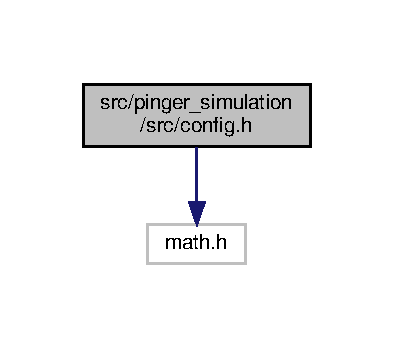
\includegraphics[width=189pt]{pinger__simulation_2src_2config_8h__incl}
\end{center}
\end{figure}
This graph shows which files directly or indirectly include this file\+:\nopagebreak
\begin{figure}[H]
\begin{center}
\leavevmode
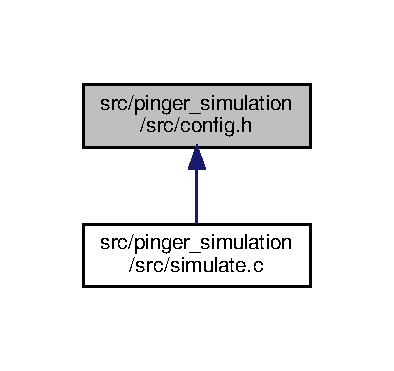
\includegraphics[width=189pt]{pinger__simulation_2src_2config_8h__dep__incl}
\end{center}
\end{figure}
\subsection*{Macros}
\begin{Indent}\textbf{ Signal receiver configuration.}\par
\begin{DoxyCompactItemize}
\item 
\#define \hyperlink{pinger__simulation_2src_2config_8h_a091fa5a1559fc7162d665edb1bed521e}{N\+U\+M\+\_\+\+P\+H\+O\+N\+ES}~4
\item 
\#define \hyperlink{pinger__simulation_2src_2config_8h_ab2dc237e07e2b4c8a52a5203c216fd37}{S\+P\+A\+C\+I\+NG}~0.\+0127
\end{DoxyCompactItemize}
\end{Indent}
\begin{Indent}\textbf{ Environment settings.}\par
\begin{DoxyCompactItemize}
\item 
\#define \hyperlink{pinger__simulation_2src_2config_8h_ac4cf4b2ab929bd23951a8676eeac086b}{C}~1480.
\item 
\#define \hyperlink{pinger__simulation_2src_2config_8h_a43b5bb333b6864dd55d19cb078885e1c}{P\+I\+N\+G\+E\+R\+\_\+\+X\+\_\+\+L\+OC}~4.
\item 
\#define \hyperlink{pinger__simulation_2src_2config_8h_a7231fef7df5233df8a66ea9ca83dd180}{P\+I\+N\+G\+E\+R\+\_\+\+Y\+\_\+\+L\+OC}~-\/1.
\item 
\#define \hyperlink{pinger__simulation_2src_2config_8h_a2ab300cbf3906ff6fcc7b07681dac361}{F0}~25000.
\item 
\#define \hyperlink{pinger__simulation_2src_2config_8h_ad41b89d4eb6d63a0def5e5fd2a5ab326}{T0}~1./\hyperlink{pinger__localization_2src_2config_8h_a5947531331b6f35777ca36c1077706b2}{F0}
\item 
\#define \hyperlink{pinger__simulation_2src_2config_8h_a1252823eae0fb4c87dddc5c2caef7790}{N\+O\+I\+SE}~0.\+0
\item 
\#define \hyperlink{pinger__simulation_2src_2config_8h_a0b9a59d58ea14eb6a111dd951c6223ff}{T\+I\+M\+E\+\_\+\+B\+E\+T\+W\+E\+E\+N\+\_\+\+P\+I\+N\+GS}~0.\+5
\item 
\#define \hyperlink{pinger__simulation_2src_2config_8h_aa7dc7eb774a66c07fe17a3fe0224fe03}{P\+I\+N\+G\+\_\+\+D\+U\+R\+A\+T\+I\+ON}~0.\+005
\end{DoxyCompactItemize}
\end{Indent}
\begin{Indent}\textbf{ Sampling settings.}\par
\begin{DoxyCompactItemize}
\item 
\#define \hyperlink{pinger__simulation_2src_2config_8h_a30588c5eca7c9cb6ebba02a0236f0119}{FS}~400000.
\item 
\#define \hyperlink{pinger__simulation_2src_2config_8h_aaade3232ef08cf18b4f3a20a0a2c6fb6}{TS}~1./\hyperlink{pinger__localization_2src_2config_8h_a7a6b19aebea6b1104b347e66042a8817}{FS}
\end{DoxyCompactItemize}
\end{Indent}


\subsection{Detailed Description}
Constants to simulate a pinger, its environment, and sampling. 

\begin{DoxyAuthor}{Author}
David Zhang (Davarco)  No known bugs. 
\end{DoxyAuthor}


\subsection{Macro Definition Documentation}
\mbox{\Hypertarget{pinger__simulation_2src_2config_8h_ac4cf4b2ab929bd23951a8676eeac086b}\label{pinger__simulation_2src_2config_8h_ac4cf4b2ab929bd23951a8676eeac086b}} 
\index{pinger\+\_\+simulation/src/config.\+h@{pinger\+\_\+simulation/src/config.\+h}!C@{C}}
\index{C@{C}!pinger\+\_\+simulation/src/config.\+h@{pinger\+\_\+simulation/src/config.\+h}}
\subsubsection{\texorpdfstring{C}{C}}
{\footnotesize\ttfamily \#define C~1480.}

Wave speed, set to speed of sound in water (m/s). \mbox{\Hypertarget{pinger__simulation_2src_2config_8h_a2ab300cbf3906ff6fcc7b07681dac361}\label{pinger__simulation_2src_2config_8h_a2ab300cbf3906ff6fcc7b07681dac361}} 
\index{pinger\+\_\+simulation/src/config.\+h@{pinger\+\_\+simulation/src/config.\+h}!F0@{F0}}
\index{F0@{F0}!pinger\+\_\+simulation/src/config.\+h@{pinger\+\_\+simulation/src/config.\+h}}
\subsubsection{\texorpdfstring{F0}{F0}}
{\footnotesize\ttfamily \#define F0~25000.}

Pinger freq (Hz). \mbox{\Hypertarget{pinger__simulation_2src_2config_8h_a30588c5eca7c9cb6ebba02a0236f0119}\label{pinger__simulation_2src_2config_8h_a30588c5eca7c9cb6ebba02a0236f0119}} 
\index{pinger\+\_\+simulation/src/config.\+h@{pinger\+\_\+simulation/src/config.\+h}!FS@{FS}}
\index{FS@{FS}!pinger\+\_\+simulation/src/config.\+h@{pinger\+\_\+simulation/src/config.\+h}}
\subsubsection{\texorpdfstring{FS}{FS}}
{\footnotesize\ttfamily \#define FS~400000.}

Sampling rate (Hz). \mbox{\Hypertarget{pinger__simulation_2src_2config_8h_a1252823eae0fb4c87dddc5c2caef7790}\label{pinger__simulation_2src_2config_8h_a1252823eae0fb4c87dddc5c2caef7790}} 
\index{pinger\+\_\+simulation/src/config.\+h@{pinger\+\_\+simulation/src/config.\+h}!N\+O\+I\+SE@{N\+O\+I\+SE}}
\index{N\+O\+I\+SE@{N\+O\+I\+SE}!pinger\+\_\+simulation/src/config.\+h@{pinger\+\_\+simulation/src/config.\+h}}
\subsubsection{\texorpdfstring{N\+O\+I\+SE}{NOISE}}
{\footnotesize\ttfamily \#define N\+O\+I\+SE~0.\+0}

Noise, expressed as a fraction of the signal (0.\+1=10\%). \mbox{\Hypertarget{pinger__simulation_2src_2config_8h_a091fa5a1559fc7162d665edb1bed521e}\label{pinger__simulation_2src_2config_8h_a091fa5a1559fc7162d665edb1bed521e}} 
\index{pinger\+\_\+simulation/src/config.\+h@{pinger\+\_\+simulation/src/config.\+h}!N\+U\+M\+\_\+\+P\+H\+O\+N\+ES@{N\+U\+M\+\_\+\+P\+H\+O\+N\+ES}}
\index{N\+U\+M\+\_\+\+P\+H\+O\+N\+ES@{N\+U\+M\+\_\+\+P\+H\+O\+N\+ES}!pinger\+\_\+simulation/src/config.\+h@{pinger\+\_\+simulation/src/config.\+h}}
\subsubsection{\texorpdfstring{N\+U\+M\+\_\+\+P\+H\+O\+N\+ES}{NUM\_PHONES}}
{\footnotesize\ttfamily \#define N\+U\+M\+\_\+\+P\+H\+O\+N\+ES~4}

Total number of signal receivers. \mbox{\Hypertarget{pinger__simulation_2src_2config_8h_aa7dc7eb774a66c07fe17a3fe0224fe03}\label{pinger__simulation_2src_2config_8h_aa7dc7eb774a66c07fe17a3fe0224fe03}} 
\index{pinger\+\_\+simulation/src/config.\+h@{pinger\+\_\+simulation/src/config.\+h}!P\+I\+N\+G\+\_\+\+D\+U\+R\+A\+T\+I\+ON@{P\+I\+N\+G\+\_\+\+D\+U\+R\+A\+T\+I\+ON}}
\index{P\+I\+N\+G\+\_\+\+D\+U\+R\+A\+T\+I\+ON@{P\+I\+N\+G\+\_\+\+D\+U\+R\+A\+T\+I\+ON}!pinger\+\_\+simulation/src/config.\+h@{pinger\+\_\+simulation/src/config.\+h}}
\subsubsection{\texorpdfstring{P\+I\+N\+G\+\_\+\+D\+U\+R\+A\+T\+I\+ON}{PING\_DURATION}}
{\footnotesize\ttfamily \#define P\+I\+N\+G\+\_\+\+D\+U\+R\+A\+T\+I\+ON~0.\+005}

Length of a ping burst (seconds). \mbox{\Hypertarget{pinger__simulation_2src_2config_8h_a43b5bb333b6864dd55d19cb078885e1c}\label{pinger__simulation_2src_2config_8h_a43b5bb333b6864dd55d19cb078885e1c}} 
\index{pinger\+\_\+simulation/src/config.\+h@{pinger\+\_\+simulation/src/config.\+h}!P\+I\+N\+G\+E\+R\+\_\+\+X\+\_\+\+L\+OC@{P\+I\+N\+G\+E\+R\+\_\+\+X\+\_\+\+L\+OC}}
\index{P\+I\+N\+G\+E\+R\+\_\+\+X\+\_\+\+L\+OC@{P\+I\+N\+G\+E\+R\+\_\+\+X\+\_\+\+L\+OC}!pinger\+\_\+simulation/src/config.\+h@{pinger\+\_\+simulation/src/config.\+h}}
\subsubsection{\texorpdfstring{P\+I\+N\+G\+E\+R\+\_\+\+X\+\_\+\+L\+OC}{PINGER\_X\_LOC}}
{\footnotesize\ttfamily \#define P\+I\+N\+G\+E\+R\+\_\+\+X\+\_\+\+L\+OC~4.}

Units north (meters). \mbox{\Hypertarget{pinger__simulation_2src_2config_8h_a7231fef7df5233df8a66ea9ca83dd180}\label{pinger__simulation_2src_2config_8h_a7231fef7df5233df8a66ea9ca83dd180}} 
\index{pinger\+\_\+simulation/src/config.\+h@{pinger\+\_\+simulation/src/config.\+h}!P\+I\+N\+G\+E\+R\+\_\+\+Y\+\_\+\+L\+OC@{P\+I\+N\+G\+E\+R\+\_\+\+Y\+\_\+\+L\+OC}}
\index{P\+I\+N\+G\+E\+R\+\_\+\+Y\+\_\+\+L\+OC@{P\+I\+N\+G\+E\+R\+\_\+\+Y\+\_\+\+L\+OC}!pinger\+\_\+simulation/src/config.\+h@{pinger\+\_\+simulation/src/config.\+h}}
\subsubsection{\texorpdfstring{P\+I\+N\+G\+E\+R\+\_\+\+Y\+\_\+\+L\+OC}{PINGER\_Y\_LOC}}
{\footnotesize\ttfamily \#define P\+I\+N\+G\+E\+R\+\_\+\+Y\+\_\+\+L\+OC~-\/1.}

Units east (meters). \mbox{\Hypertarget{pinger__simulation_2src_2config_8h_ab2dc237e07e2b4c8a52a5203c216fd37}\label{pinger__simulation_2src_2config_8h_ab2dc237e07e2b4c8a52a5203c216fd37}} 
\index{pinger\+\_\+simulation/src/config.\+h@{pinger\+\_\+simulation/src/config.\+h}!S\+P\+A\+C\+I\+NG@{S\+P\+A\+C\+I\+NG}}
\index{S\+P\+A\+C\+I\+NG@{S\+P\+A\+C\+I\+NG}!pinger\+\_\+simulation/src/config.\+h@{pinger\+\_\+simulation/src/config.\+h}}
\subsubsection{\texorpdfstring{S\+P\+A\+C\+I\+NG}{SPACING}}
{\footnotesize\ttfamily \#define S\+P\+A\+C\+I\+NG~0.\+0127}

Spacing between two signal receivers. \mbox{\Hypertarget{pinger__simulation_2src_2config_8h_ad41b89d4eb6d63a0def5e5fd2a5ab326}\label{pinger__simulation_2src_2config_8h_ad41b89d4eb6d63a0def5e5fd2a5ab326}} 
\index{pinger\+\_\+simulation/src/config.\+h@{pinger\+\_\+simulation/src/config.\+h}!T0@{T0}}
\index{T0@{T0}!pinger\+\_\+simulation/src/config.\+h@{pinger\+\_\+simulation/src/config.\+h}}
\subsubsection{\texorpdfstring{T0}{T0}}
{\footnotesize\ttfamily \#define T0~1./\hyperlink{pinger__localization_2src_2config_8h_a5947531331b6f35777ca36c1077706b2}{F0}}

Pinger period (seconds). \mbox{\Hypertarget{pinger__simulation_2src_2config_8h_a0b9a59d58ea14eb6a111dd951c6223ff}\label{pinger__simulation_2src_2config_8h_a0b9a59d58ea14eb6a111dd951c6223ff}} 
\index{pinger\+\_\+simulation/src/config.\+h@{pinger\+\_\+simulation/src/config.\+h}!T\+I\+M\+E\+\_\+\+B\+E\+T\+W\+E\+E\+N\+\_\+\+P\+I\+N\+GS@{T\+I\+M\+E\+\_\+\+B\+E\+T\+W\+E\+E\+N\+\_\+\+P\+I\+N\+GS}}
\index{T\+I\+M\+E\+\_\+\+B\+E\+T\+W\+E\+E\+N\+\_\+\+P\+I\+N\+GS@{T\+I\+M\+E\+\_\+\+B\+E\+T\+W\+E\+E\+N\+\_\+\+P\+I\+N\+GS}!pinger\+\_\+simulation/src/config.\+h@{pinger\+\_\+simulation/src/config.\+h}}
\subsubsection{\texorpdfstring{T\+I\+M\+E\+\_\+\+B\+E\+T\+W\+E\+E\+N\+\_\+\+P\+I\+N\+GS}{TIME\_BETWEEN\_PINGS}}
{\footnotesize\ttfamily \#define T\+I\+M\+E\+\_\+\+B\+E\+T\+W\+E\+E\+N\+\_\+\+P\+I\+N\+GS~0.\+5}

Amount of time pinger is silent per burst (seconds). \mbox{\Hypertarget{pinger__simulation_2src_2config_8h_aaade3232ef08cf18b4f3a20a0a2c6fb6}\label{pinger__simulation_2src_2config_8h_aaade3232ef08cf18b4f3a20a0a2c6fb6}} 
\index{pinger\+\_\+simulation/src/config.\+h@{pinger\+\_\+simulation/src/config.\+h}!TS@{TS}}
\index{TS@{TS}!pinger\+\_\+simulation/src/config.\+h@{pinger\+\_\+simulation/src/config.\+h}}
\subsubsection{\texorpdfstring{TS}{TS}}
{\footnotesize\ttfamily \#define TS~1./\hyperlink{pinger__localization_2src_2config_8h_a7a6b19aebea6b1104b347e66042a8817}{FS}}

Sampling period (seconds). 
\hypertarget{main_8c}{}\section{src/pinger\+\_\+localization/src/main.c File Reference}
\label{main_8c}\index{src/pinger\+\_\+localization/src/main.\+c@{src/pinger\+\_\+localization/src/main.\+c}}


Runs M\+U\+S\+IC for an acoustic localization system.  


{\ttfamily \#include $<$stdio.\+h$>$}\newline
{\ttfamily \#include $<$stdlib.\+h$>$}\newline
{\ttfamily \#include $<$math.\+h$>$}\newline
{\ttfamily \#include \char`\"{}music.\+h\char`\"{}}\newline
{\ttfamily \#include \char`\"{}config.\+h\char`\"{}}\newline
{\ttfamily \#include \char`\"{}matrix.\+h\char`\"{}}\newline
Include dependency graph for main.\+c\+:\nopagebreak
\begin{figure}[H]
\begin{center}
\leavevmode
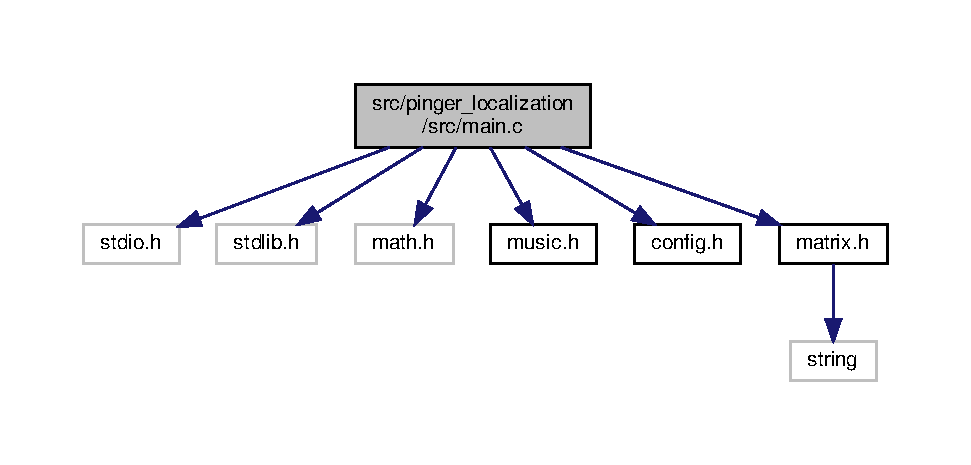
\includegraphics[width=350pt]{main_8c__incl}
\end{center}
\end{figure}
\subsection*{Functions}
\begin{DoxyCompactItemize}
\item 
\mbox{\Hypertarget{main_8c_ae66f6b31b5ad750f1fe042a706a4e3d4}\label{main_8c_ae66f6b31b5ad750f1fe042a706a4e3d4}} 
int {\bfseries main} ()
\end{DoxyCompactItemize}


\subsection{Detailed Description}
Runs M\+U\+S\+IC for an acoustic localization system. 

\begin{DoxyAuthor}{Author}
David Zhang (Davarco) 
\end{DoxyAuthor}

\hypertarget{matrix_8c}{}\section{src/pinger\+\_\+localization/src/matrix.c File Reference}
\label{matrix_8c}\index{src/pinger\+\_\+localization/src/matrix.\+c@{src/pinger\+\_\+localization/src/matrix.\+c}}


Functions used for real and complex matrix operations.  


{\ttfamily \#include $<$stdio.\+h$>$}\newline
{\ttfamily \#include $<$math.\+h$>$}\newline
{\ttfamily \#include \char`\"{}matrix.\+h\char`\"{}}\newline
Include dependency graph for matrix.\+c\+:
\nopagebreak
\begin{figure}[H]
\begin{center}
\leavevmode
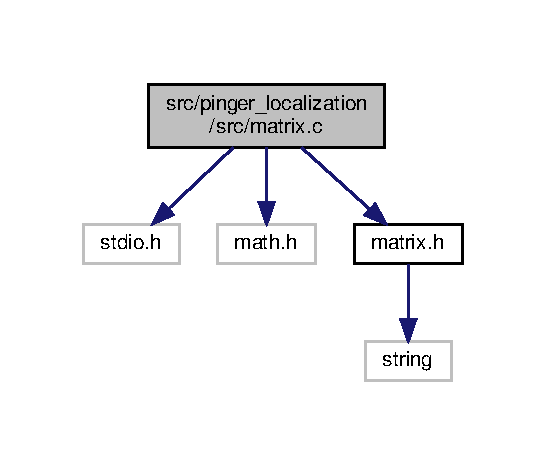
\includegraphics[width=262pt]{matrix_8c__incl}
\end{center}
\end{figure}
\subsection*{Functions}
\begin{DoxyCompactItemize}
\item 
void \hyperlink{matrix_8c_a81c96d873cc9c72c183277f3318b9488}{print} (double $\ast$A, int m, int n, char $\ast$msg)
\begin{DoxyCompactList}\small\item\em Print real matrix to terminal. \end{DoxyCompactList}\item 
void \hyperlink{matrix_8c_a078e23ec05fcd85756bc7f635cdc530d}{print\+\_\+complex} (double $\ast$Ar, double $\ast$Ai, int m, int n, char $\ast$msg)
\begin{DoxyCompactList}\small\item\em Print complex matrix to terminal. \end{DoxyCompactList}\item 
void \hyperlink{matrix_8c_a0c767e9d2827cc3ac53da5272dfab3ca}{identity} (double $\ast$A, int n)
\begin{DoxyCompactList}\small\item\em Create an identity matrix of order nxn. \end{DoxyCompactList}\item 
void \hyperlink{matrix_8c_a347b1b98c0fa015d4d588fcee0332043}{copy} (double $\ast$A, int m, int n, double $\ast$B)
\begin{DoxyCompactList}\small\item\em Copies the elements from one matrix to another. \end{DoxyCompactList}\item 
void \hyperlink{matrix_8c_acbe5a7b7148849089ee154afefe99898}{product} (double $\ast$A, double $\ast$B, int m, int p, int n, double $\ast$C)
\begin{DoxyCompactList}\small\item\em Multiplies two matrices together. \end{DoxyCompactList}\item 
void \hyperlink{matrix_8c_a0c46c37f20473cbb1f1f2e3c82519e65}{product\+\_\+complex} (double $\ast$Ar, double $\ast$Ai, double $\ast$Br, double $\ast$Bi, int m, int p, int n, double $\ast$Cr, double $\ast$Ci)
\begin{DoxyCompactList}\small\item\em Multiplies two complex matrices together. \end{DoxyCompactList}\item 
void \hyperlink{matrix_8c_adb13c652887fd0e887c88d53d9f4b323}{add} (double $\ast$A, double $\ast$B, int m, int n, double $\ast$C)
\begin{DoxyCompactList}\small\item\em Adds two matrices together. \end{DoxyCompactList}\item 
void \hyperlink{matrix_8c_ab67f48f8dfa82239b1f5dfd90aad2c1d}{subtract} (double $\ast$A, double $\ast$B, int m, int n, double $\ast$C)
\begin{DoxyCompactList}\small\item\em Subtracts two matrices. \end{DoxyCompactList}\item 
void \hyperlink{matrix_8c_a296d2426aeb7a46d455ce46f47d97eb9}{transpose} (double $\ast$A, int m, int n, double $\ast$B)
\begin{DoxyCompactList}\small\item\em Takes the transpose of a matrix. \end{DoxyCompactList}\item 
void \hyperlink{matrix_8c_af968034cbd25008e068ad06c1daa5cfe}{transpose\+\_\+complex} (double $\ast$Ar, double $\ast$Ai, int m, int n, double $\ast$Br, double $\ast$Bi)
\begin{DoxyCompactList}\small\item\em Takes the transpose (complex conjugate) of a complex matrix. \end{DoxyCompactList}\item 
void \hyperlink{matrix_8c_ab5b944d92518695545660022e285fce6}{scale} (double $\ast$A, int m, int n, double a)
\begin{DoxyCompactList}\small\item\em Multiplies a matrix by a scalar. \end{DoxyCompactList}\item 
void \hyperlink{matrix_8c_a4a7fcecfbdb3cf01665981c858dd5984}{slice} (double $\ast$A, int n, int m1, int m2, int n1, int n2, double $\ast$B)
\begin{DoxyCompactList}\small\item\em Slices a matrix. \end{DoxyCompactList}\item 
void \hyperlink{matrix_8c_ad58cbef9da2956cfcb53e1e9f361b61f}{inverse} (double $\ast$A, int n, double $\ast$B)
\begin{DoxyCompactList}\small\item\em Takes the inverse of a matrix. \end{DoxyCompactList}\item 
void \hyperlink{matrix_8c_a74c8fe363560854e31ccc3862fa00e8b}{eigen} (double $\ast$A, int n, double $\ast$val, double $\ast$vec)
\begin{DoxyCompactList}\small\item\em Takes the eigenvalues and eigenvectors of a real matrix. \end{DoxyCompactList}\item 
void \hyperlink{matrix_8c_ab429c38bf9e0188c44427627e1f692f0}{eigen\+\_\+complex} (double $\ast$Ar, double $\ast$Ai, int n, double $\ast$val, double $\ast$vecr, double $\ast$veci)
\begin{DoxyCompactList}\small\item\em Takes the eigenvalues and eigenvectors of a complex matrix. \end{DoxyCompactList}\end{DoxyCompactItemize}


\subsection{Detailed Description}
Functions used for real and complex matrix operations. 

\begin{DoxyAuthor}{Author}
David Zhang (Davarco) 
\end{DoxyAuthor}


\subsection{Function Documentation}
\mbox{\Hypertarget{matrix_8c_adb13c652887fd0e887c88d53d9f4b323}\label{matrix_8c_adb13c652887fd0e887c88d53d9f4b323}} 
\index{matrix.\+c@{matrix.\+c}!add@{add}}
\index{add@{add}!matrix.\+c@{matrix.\+c}}
\subsubsection{\texorpdfstring{add()}{add()}}
{\footnotesize\ttfamily void add (\begin{DoxyParamCaption}\item[{double $\ast$}]{A,  }\item[{double $\ast$}]{B,  }\item[{int}]{m,  }\item[{int}]{n,  }\item[{double $\ast$}]{C }\end{DoxyParamCaption})}



Adds two matrices together. 


\begin{DoxyParams}{Parameters}
{\em A} & The first matrix. \\
\hline
{\em B} & The second matrix. \\
\hline
{\em m} & The number of rows in A and B. \\
\hline
{\em n} & The number of columns in A and B. \\
\hline
{\em C} & The added matrix. \\
\hline
\end{DoxyParams}
\begin{DoxyReturn}{Returns}
Void. 
\end{DoxyReturn}
\mbox{\Hypertarget{matrix_8c_a347b1b98c0fa015d4d588fcee0332043}\label{matrix_8c_a347b1b98c0fa015d4d588fcee0332043}} 
\index{matrix.\+c@{matrix.\+c}!copy@{copy}}
\index{copy@{copy}!matrix.\+c@{matrix.\+c}}
\subsubsection{\texorpdfstring{copy()}{copy()}}
{\footnotesize\ttfamily void copy (\begin{DoxyParamCaption}\item[{double $\ast$}]{A,  }\item[{int}]{m,  }\item[{int}]{n,  }\item[{double $\ast$}]{B }\end{DoxyParamCaption})}



Copies the elements from one matrix to another. 


\begin{DoxyParams}{Parameters}
{\em A} & The matrix from where elements are copied from. \\
\hline
{\em m} & The number of rows in A and B. \\
\hline
{\em n} & The number of columns in A and B. \\
\hline
{\em B} & The matrix where elements are written to. \\
\hline
\end{DoxyParams}
\begin{DoxyReturn}{Returns}
Void. 
\end{DoxyReturn}
\mbox{\Hypertarget{matrix_8c_a74c8fe363560854e31ccc3862fa00e8b}\label{matrix_8c_a74c8fe363560854e31ccc3862fa00e8b}} 
\index{matrix.\+c@{matrix.\+c}!eigen@{eigen}}
\index{eigen@{eigen}!matrix.\+c@{matrix.\+c}}
\subsubsection{\texorpdfstring{eigen()}{eigen()}}
{\footnotesize\ttfamily void eigen (\begin{DoxyParamCaption}\item[{double $\ast$}]{A,  }\item[{int}]{n,  }\item[{double $\ast$}]{val,  }\item[{double $\ast$}]{vec }\end{DoxyParamCaption})}



Takes the eigenvalues and eigenvectors of a real matrix. 


\begin{DoxyParams}{Parameters}
{\em A} & The input matrix, must be square. \\
\hline
{\em n} & The number of rows and columns in A. \\
\hline
{\em val} & The address where the eigenvalues are stored. \\
\hline
{\em vec} & The address where the eigenvectors are stored. \\
\hline
\end{DoxyParams}
\begin{DoxyReturn}{Returns}
Void. 
\end{DoxyReturn}
\mbox{\Hypertarget{matrix_8c_ab429c38bf9e0188c44427627e1f692f0}\label{matrix_8c_ab429c38bf9e0188c44427627e1f692f0}} 
\index{matrix.\+c@{matrix.\+c}!eigen\+\_\+complex@{eigen\+\_\+complex}}
\index{eigen\+\_\+complex@{eigen\+\_\+complex}!matrix.\+c@{matrix.\+c}}
\subsubsection{\texorpdfstring{eigen\+\_\+complex()}{eigen\_complex()}}
{\footnotesize\ttfamily void eigen\+\_\+complex (\begin{DoxyParamCaption}\item[{double $\ast$}]{Ar,  }\item[{double $\ast$}]{Ai,  }\item[{int}]{n,  }\item[{double $\ast$}]{val,  }\item[{double $\ast$}]{vecr,  }\item[{double $\ast$}]{veci }\end{DoxyParamCaption})}



Takes the eigenvalues and eigenvectors of a complex matrix. 


\begin{DoxyParams}{Parameters}
{\em Ar} & The real components of the input matrix. \\
\hline
{\em Ai} & The imaginary components of the input matrix. \\
\hline
{\em n} & The number of rows and columns in A. \\
\hline
{\em val} & The address where the eigenvalues are stored. \\
\hline
{\em vecr} & The address for the real components of the eigenvectors. \\
\hline
{\em veci} & The address for the imaginary components of the eigenvectors. \\
\hline
\end{DoxyParams}
\begin{DoxyReturn}{Returns}
Void. 
\end{DoxyReturn}
\mbox{\Hypertarget{matrix_8c_a0c767e9d2827cc3ac53da5272dfab3ca}\label{matrix_8c_a0c767e9d2827cc3ac53da5272dfab3ca}} 
\index{matrix.\+c@{matrix.\+c}!identity@{identity}}
\index{identity@{identity}!matrix.\+c@{matrix.\+c}}
\subsubsection{\texorpdfstring{identity()}{identity()}}
{\footnotesize\ttfamily void identity (\begin{DoxyParamCaption}\item[{double $\ast$}]{A,  }\item[{int}]{n }\end{DoxyParamCaption})}



Create an identity matrix of order nxn. 


\begin{DoxyParams}{Parameters}
{\em A} & The address where the matrix is written. \\
\hline
{\em n} & The number of rows and columns of A. \\
\hline
\end{DoxyParams}
\begin{DoxyReturn}{Returns}
Void. 
\end{DoxyReturn}
\mbox{\Hypertarget{matrix_8c_ad58cbef9da2956cfcb53e1e9f361b61f}\label{matrix_8c_ad58cbef9da2956cfcb53e1e9f361b61f}} 
\index{matrix.\+c@{matrix.\+c}!inverse@{inverse}}
\index{inverse@{inverse}!matrix.\+c@{matrix.\+c}}
\subsubsection{\texorpdfstring{inverse()}{inverse()}}
{\footnotesize\ttfamily void inverse (\begin{DoxyParamCaption}\item[{double $\ast$}]{A,  }\item[{int}]{n,  }\item[{double $\ast$}]{B }\end{DoxyParamCaption})}



Takes the inverse of a matrix. 


\begin{DoxyParams}{Parameters}
{\em A} & The input matrix, must be square. \\
\hline
{\em n} & The number of rows and columns in A. \\
\hline
{\em B} & The inverted matrix. \\
\hline
\end{DoxyParams}
\begin{DoxyReturn}{Returns}
Void. 
\end{DoxyReturn}
\mbox{\Hypertarget{matrix_8c_a81c96d873cc9c72c183277f3318b9488}\label{matrix_8c_a81c96d873cc9c72c183277f3318b9488}} 
\index{matrix.\+c@{matrix.\+c}!print@{print}}
\index{print@{print}!matrix.\+c@{matrix.\+c}}
\subsubsection{\texorpdfstring{print()}{print()}}
{\footnotesize\ttfamily void print (\begin{DoxyParamCaption}\item[{double $\ast$}]{A,  }\item[{int}]{m,  }\item[{int}]{n,  }\item[{char $\ast$}]{msg }\end{DoxyParamCaption})}



Print real matrix to terminal. 


\begin{DoxyParams}{Parameters}
{\em A} & The matrix that is printed. \\
\hline
{\em m} & The number of rows in A. \\
\hline
{\em n} & The number of columns in B. \\
\hline
{\em msg} & The header message preceding the matrix. \\
\hline
\end{DoxyParams}
\begin{DoxyReturn}{Returns}
Void. 
\end{DoxyReturn}
\mbox{\Hypertarget{matrix_8c_a078e23ec05fcd85756bc7f635cdc530d}\label{matrix_8c_a078e23ec05fcd85756bc7f635cdc530d}} 
\index{matrix.\+c@{matrix.\+c}!print\+\_\+complex@{print\+\_\+complex}}
\index{print\+\_\+complex@{print\+\_\+complex}!matrix.\+c@{matrix.\+c}}
\subsubsection{\texorpdfstring{print\+\_\+complex()}{print\_complex()}}
{\footnotesize\ttfamily void print\+\_\+complex (\begin{DoxyParamCaption}\item[{double $\ast$}]{Ar,  }\item[{double $\ast$}]{Ai,  }\item[{int}]{m,  }\item[{int}]{n,  }\item[{char $\ast$}]{msg }\end{DoxyParamCaption})}



Print complex matrix to terminal. 


\begin{DoxyParams}{Parameters}
{\em Ar} & The real components of the matrix that is printed. \\
\hline
{\em Ai} & The imaginary components of the matrix that is printed. \\
\hline
{\em m} & The number of rows in Ar and Ai. \\
\hline
{\em n} & The number of columns in Br and Bi. \\
\hline
{\em msg} & The header message preceding the matrix. \\
\hline
\end{DoxyParams}
\begin{DoxyReturn}{Returns}
Void. 
\end{DoxyReturn}
\mbox{\Hypertarget{matrix_8c_acbe5a7b7148849089ee154afefe99898}\label{matrix_8c_acbe5a7b7148849089ee154afefe99898}} 
\index{matrix.\+c@{matrix.\+c}!product@{product}}
\index{product@{product}!matrix.\+c@{matrix.\+c}}
\subsubsection{\texorpdfstring{product()}{product()}}
{\footnotesize\ttfamily void product (\begin{DoxyParamCaption}\item[{double $\ast$}]{A,  }\item[{double $\ast$}]{B,  }\item[{int}]{m,  }\item[{int}]{p,  }\item[{int}]{n,  }\item[{double $\ast$}]{C }\end{DoxyParamCaption})}



Multiplies two matrices together. 


\begin{DoxyParams}{Parameters}
{\em A} & The first matrix. \\
\hline
{\em B} & The second matrix. \\
\hline
{\em m} & The number of rows in A. \\
\hline
{\em p} & The number of columns in A and number of rows in B. \\
\hline
{\em n} & The number of columns in B. \\
\hline
{\em C} & The multiplied matrix of order mxn. \\
\hline
\end{DoxyParams}
\begin{DoxyReturn}{Returns}
Void. 
\end{DoxyReturn}
\mbox{\Hypertarget{matrix_8c_a0c46c37f20473cbb1f1f2e3c82519e65}\label{matrix_8c_a0c46c37f20473cbb1f1f2e3c82519e65}} 
\index{matrix.\+c@{matrix.\+c}!product\+\_\+complex@{product\+\_\+complex}}
\index{product\+\_\+complex@{product\+\_\+complex}!matrix.\+c@{matrix.\+c}}
\subsubsection{\texorpdfstring{product\+\_\+complex()}{product\_complex()}}
{\footnotesize\ttfamily void product\+\_\+complex (\begin{DoxyParamCaption}\item[{double $\ast$}]{Ar,  }\item[{double $\ast$}]{Ai,  }\item[{double $\ast$}]{Br,  }\item[{double $\ast$}]{Bi,  }\item[{int}]{m,  }\item[{int}]{p,  }\item[{int}]{n,  }\item[{double $\ast$}]{Cr,  }\item[{double $\ast$}]{Ci }\end{DoxyParamCaption})}



Multiplies two complex matrices together. 


\begin{DoxyParams}{Parameters}
{\em Ar} & The real components of the first matrix. \\
\hline
{\em Ai} & The imaginary components of the first matrix. \\
\hline
{\em Br} & The real components of the second matrix. \\
\hline
{\em Bi} & The imaginary components of the second matrix. \\
\hline
{\em m} & The number of rows in A. \\
\hline
{\em p} & The number of columns in A and number of rows in B. \\
\hline
{\em n} & The number of columns in B. \\
\hline
{\em Cr} & The real components of the multiplied matrix. \\
\hline
{\em Ci} & The imaginary components of the multiplied matrix. \\
\hline
\end{DoxyParams}
\begin{DoxyReturn}{Returns}
Void. 
\end{DoxyReturn}
\mbox{\Hypertarget{matrix_8c_ab5b944d92518695545660022e285fce6}\label{matrix_8c_ab5b944d92518695545660022e285fce6}} 
\index{matrix.\+c@{matrix.\+c}!scale@{scale}}
\index{scale@{scale}!matrix.\+c@{matrix.\+c}}
\subsubsection{\texorpdfstring{scale()}{scale()}}
{\footnotesize\ttfamily void scale (\begin{DoxyParamCaption}\item[{double $\ast$}]{A,  }\item[{int}]{m,  }\item[{int}]{n,  }\item[{double}]{k }\end{DoxyParamCaption})}



Multiplies a matrix by a scalar. 


\begin{DoxyParams}{Parameters}
{\em A} & The input matrix, where the results are written to as well. \\
\hline
{\em m} & The number of rows in A. \\
\hline
{\em n} & The number of columns in A. \\
\hline
{\em k} & The scalar value. \\
\hline
\end{DoxyParams}
\begin{DoxyReturn}{Returns}
Void. 
\end{DoxyReturn}
\mbox{\Hypertarget{matrix_8c_a4a7fcecfbdb3cf01665981c858dd5984}\label{matrix_8c_a4a7fcecfbdb3cf01665981c858dd5984}} 
\index{matrix.\+c@{matrix.\+c}!slice@{slice}}
\index{slice@{slice}!matrix.\+c@{matrix.\+c}}
\subsubsection{\texorpdfstring{slice()}{slice()}}
{\footnotesize\ttfamily void slice (\begin{DoxyParamCaption}\item[{double $\ast$}]{A,  }\item[{int}]{n,  }\item[{int}]{m1,  }\item[{int}]{m2,  }\item[{int}]{n1,  }\item[{int}]{n2,  }\item[{double $\ast$}]{B }\end{DoxyParamCaption})}



Slices a matrix. 

The sliced matrix is equal to A\mbox{[}m1\+:m2-\/1, n1\+:n2-\/1\mbox{]}.


\begin{DoxyParams}{Parameters}
{\em A} & The input matrix. \\
\hline
{\em n} & The number of columns in A. \\
\hline
{\em m1} & The first row to slice from. \\
\hline
{\em m2} & The row after the stop slicing at. \\
\hline
{\em n1} & The first column to slice from. \\
\hline
{\em n2} & The column after the stop slicing at. \\
\hline
{\em B} & The sliced matrix. \\
\hline
\end{DoxyParams}
\begin{DoxyReturn}{Returns}
Void. 
\end{DoxyReturn}
\mbox{\Hypertarget{matrix_8c_ab67f48f8dfa82239b1f5dfd90aad2c1d}\label{matrix_8c_ab67f48f8dfa82239b1f5dfd90aad2c1d}} 
\index{matrix.\+c@{matrix.\+c}!subtract@{subtract}}
\index{subtract@{subtract}!matrix.\+c@{matrix.\+c}}
\subsubsection{\texorpdfstring{subtract()}{subtract()}}
{\footnotesize\ttfamily void subtract (\begin{DoxyParamCaption}\item[{double $\ast$}]{A,  }\item[{double $\ast$}]{B,  }\item[{int}]{m,  }\item[{int}]{n,  }\item[{double $\ast$}]{C }\end{DoxyParamCaption})}



Subtracts two matrices. 


\begin{DoxyParams}{Parameters}
{\em A} & The first matrix. \\
\hline
{\em B} & The second matrix. \\
\hline
{\em m} & The number of rows in A and B. \\
\hline
{\em n} & The number of columns in A and B. \\
\hline
{\em C} & The subtracted matrix. \\
\hline
\end{DoxyParams}
\begin{DoxyReturn}{Returns}
Void. 
\end{DoxyReturn}
\mbox{\Hypertarget{matrix_8c_a296d2426aeb7a46d455ce46f47d97eb9}\label{matrix_8c_a296d2426aeb7a46d455ce46f47d97eb9}} 
\index{matrix.\+c@{matrix.\+c}!transpose@{transpose}}
\index{transpose@{transpose}!matrix.\+c@{matrix.\+c}}
\subsubsection{\texorpdfstring{transpose()}{transpose()}}
{\footnotesize\ttfamily void transpose (\begin{DoxyParamCaption}\item[{double $\ast$}]{A,  }\item[{int}]{m,  }\item[{int}]{n,  }\item[{double $\ast$}]{B }\end{DoxyParamCaption})}



Takes the transpose of a matrix. 


\begin{DoxyParams}{Parameters}
{\em A} & The input matrix to transpose. \\
\hline
{\em m} & The number of rows in A. \\
\hline
{\em n} & The number of columns in A. \\
\hline
{\em B} & The transposed matrix of order nxm. \\
\hline
\end{DoxyParams}
\begin{DoxyReturn}{Returns}
Void. 
\end{DoxyReturn}
\mbox{\Hypertarget{matrix_8c_af968034cbd25008e068ad06c1daa5cfe}\label{matrix_8c_af968034cbd25008e068ad06c1daa5cfe}} 
\index{matrix.\+c@{matrix.\+c}!transpose\+\_\+complex@{transpose\+\_\+complex}}
\index{transpose\+\_\+complex@{transpose\+\_\+complex}!matrix.\+c@{matrix.\+c}}
\subsubsection{\texorpdfstring{transpose\+\_\+complex()}{transpose\_complex()}}
{\footnotesize\ttfamily void transpose\+\_\+complex (\begin{DoxyParamCaption}\item[{double $\ast$}]{Ar,  }\item[{double $\ast$}]{Ai,  }\item[{int}]{m,  }\item[{int}]{n,  }\item[{double $\ast$}]{Br,  }\item[{double $\ast$}]{Bi }\end{DoxyParamCaption})}



Takes the transpose (complex conjugate) of a complex matrix. 


\begin{DoxyParams}{Parameters}
{\em Ar} & The real components of the first matrix. \\
\hline
{\em Ai} & The imaginary components of the first matrix. \\
\hline
{\em m} & The number of rows in A. \\
\hline
{\em n} & The number of columns in B. \\
\hline
{\em Br} & The real components of the transposed matrix. \\
\hline
{\em Bi} & The imaginary components of the transposed matrix. \\
\hline
\end{DoxyParams}
\begin{DoxyReturn}{Returns}
Void. 
\end{DoxyReturn}

\hypertarget{matrix_8h}{}\section{src/pinger\+\_\+localization/src/matrix.h File Reference}
\label{matrix_8h}\index{src/pinger\+\_\+localization/src/matrix.\+h@{src/pinger\+\_\+localization/src/matrix.\+h}}


Function declarations for real and complex matrix operations.  


{\ttfamily \#include $<$string$>$}\newline
Include dependency graph for matrix.\+h\+:\nopagebreak
\begin{figure}[H]
\begin{center}
\leavevmode
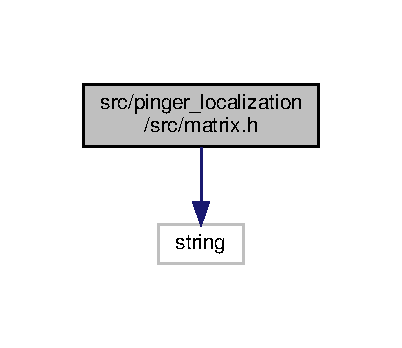
\includegraphics[width=193pt]{matrix_8h__incl}
\end{center}
\end{figure}
This graph shows which files directly or indirectly include this file\+:\nopagebreak
\begin{figure}[H]
\begin{center}
\leavevmode
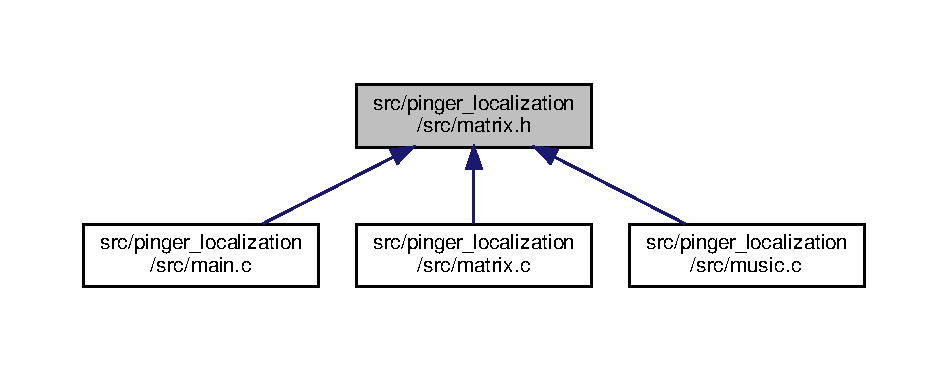
\includegraphics[width=350pt]{matrix_8h__dep__incl}
\end{center}
\end{figure}
\subsection*{Functions}
\begin{DoxyCompactItemize}
\item 
void \hyperlink{matrix_8h_a81c96d873cc9c72c183277f3318b9488}{print} (double $\ast$A, int m, int n, char $\ast$msg)
\begin{DoxyCompactList}\small\item\em Print real matrix to terminal. \end{DoxyCompactList}\item 
void \hyperlink{matrix_8h_a078e23ec05fcd85756bc7f635cdc530d}{print\+\_\+complex} (double $\ast$Ar, double $\ast$Ai, int m, int n, char $\ast$msg)
\begin{DoxyCompactList}\small\item\em Print complex matrix to terminal. \end{DoxyCompactList}\item 
void \hyperlink{matrix_8h_a0c767e9d2827cc3ac53da5272dfab3ca}{identity} (double $\ast$A, int n)
\begin{DoxyCompactList}\small\item\em Create an identity matrix of order nxn. \end{DoxyCompactList}\item 
void \hyperlink{matrix_8h_a347b1b98c0fa015d4d588fcee0332043}{copy} (double $\ast$A, int m, int n, double $\ast$B)
\begin{DoxyCompactList}\small\item\em Copies the elements from one matrix to another. \end{DoxyCompactList}\item 
void \hyperlink{matrix_8h_acbe5a7b7148849089ee154afefe99898}{product} (double $\ast$A, double $\ast$B, int m, int p, int n, double $\ast$\hyperlink{pinger__localization_2src_2config_8h_a9e8a46a0e00368ad98642587ca4ebdbe}{C})
\begin{DoxyCompactList}\small\item\em Multiplies two matrices together. \end{DoxyCompactList}\item 
void \hyperlink{matrix_8h_a0c46c37f20473cbb1f1f2e3c82519e65}{product\+\_\+complex} (double $\ast$Ar, double $\ast$Ai, double $\ast$Br, double $\ast$Bi, int m, int p, int n, double $\ast$Cr, double $\ast$Ci)
\begin{DoxyCompactList}\small\item\em Multiplies two complex matrices together. \end{DoxyCompactList}\item 
void \hyperlink{matrix_8h_adb13c652887fd0e887c88d53d9f4b323}{add} (double $\ast$A, double $\ast$B, int m, int n, double $\ast$\hyperlink{pinger__localization_2src_2config_8h_a9e8a46a0e00368ad98642587ca4ebdbe}{C})
\begin{DoxyCompactList}\small\item\em Adds two matrices together. \end{DoxyCompactList}\item 
void \hyperlink{matrix_8h_ab67f48f8dfa82239b1f5dfd90aad2c1d}{subtract} (double $\ast$A, double $\ast$B, int m, int n, double $\ast$\hyperlink{pinger__localization_2src_2config_8h_a9e8a46a0e00368ad98642587ca4ebdbe}{C})
\begin{DoxyCompactList}\small\item\em Subtracts two matrices. \end{DoxyCompactList}\item 
void \hyperlink{matrix_8h_a296d2426aeb7a46d455ce46f47d97eb9}{transpose} (double $\ast$A, int m, int n, double $\ast$B)
\begin{DoxyCompactList}\small\item\em Takes the transpose of a matrix. \end{DoxyCompactList}\item 
void \hyperlink{matrix_8h_af968034cbd25008e068ad06c1daa5cfe}{transpose\+\_\+complex} (double $\ast$Ar, double $\ast$Ai, int m, int n, double $\ast$Br, double $\ast$Bi)
\begin{DoxyCompactList}\small\item\em Takes the transpose (complex conjugate) of a complex matrix. \end{DoxyCompactList}\item 
void \hyperlink{matrix_8h_a320be7f5a43b1820a83eca703ffe5897}{scale} (double $\ast$A, int m, int n, double k)
\begin{DoxyCompactList}\small\item\em Multiplies a matrix by a scalar. \end{DoxyCompactList}\item 
void \hyperlink{matrix_8h_a4a7fcecfbdb3cf01665981c858dd5984}{slice} (double $\ast$A, int n, int m1, int m2, int n1, int n2, double $\ast$B)
\begin{DoxyCompactList}\small\item\em Slices a matrix. \end{DoxyCompactList}\item 
void \hyperlink{matrix_8h_ad58cbef9da2956cfcb53e1e9f361b61f}{inverse} (double $\ast$A, int n, double $\ast$B)
\begin{DoxyCompactList}\small\item\em Takes the inverse of a matrix. \end{DoxyCompactList}\item 
void \hyperlink{matrix_8h_a74c8fe363560854e31ccc3862fa00e8b}{eigen} (double $\ast$A, int n, double $\ast$val, double $\ast$vec)
\begin{DoxyCompactList}\small\item\em Takes the eigenvalues and eigenvectors of a real matrix. \end{DoxyCompactList}\item 
void \hyperlink{matrix_8h_ab429c38bf9e0188c44427627e1f692f0}{eigen\+\_\+complex} (double $\ast$Ar, double $\ast$Ai, int n, double $\ast$val, double $\ast$vecr, double $\ast$veci)
\begin{DoxyCompactList}\small\item\em Takes the eigenvalues and eigenvectors of a complex matrix. \end{DoxyCompactList}\end{DoxyCompactItemize}


\subsection{Detailed Description}
Function declarations for real and complex matrix operations. 

Matrices are stored in 1-\/D arrays. To access a cell, use \mbox{[}r$\ast$n+c\mbox{]} instead of \mbox{[}r\mbox{]}\mbox{[}c\mbox{]}.

Most of the other parts don\textquotesingle{}t require explanation, except for how complex matrices are handled. To create a complex matrix of order MxN, create two matrices of the same order. Use the first matrix to hold real components and the other to hold imaginary components.

\begin{DoxyAuthor}{Author}
David Zhang (Davarco) 
\end{DoxyAuthor}


\subsection{Function Documentation}
\mbox{\Hypertarget{matrix_8h_adb13c652887fd0e887c88d53d9f4b323}\label{matrix_8h_adb13c652887fd0e887c88d53d9f4b323}} 
\index{matrix.\+h@{matrix.\+h}!add@{add}}
\index{add@{add}!matrix.\+h@{matrix.\+h}}
\subsubsection{\texorpdfstring{add()}{add()}}
{\footnotesize\ttfamily void add (\begin{DoxyParamCaption}\item[{double $\ast$}]{A,  }\item[{double $\ast$}]{B,  }\item[{int}]{m,  }\item[{int}]{n,  }\item[{double $\ast$}]{C }\end{DoxyParamCaption})}



Adds two matrices together. 


\begin{DoxyParams}{Parameters}
{\em A} & The first matrix. \\
\hline
{\em B} & The second matrix. \\
\hline
{\em m} & The number of rows in A and B. \\
\hline
{\em n} & The number of columns in A and B. \\
\hline
{\em C} & The added matrix. \\
\hline
\end{DoxyParams}
\mbox{\Hypertarget{matrix_8h_a347b1b98c0fa015d4d588fcee0332043}\label{matrix_8h_a347b1b98c0fa015d4d588fcee0332043}} 
\index{matrix.\+h@{matrix.\+h}!copy@{copy}}
\index{copy@{copy}!matrix.\+h@{matrix.\+h}}
\subsubsection{\texorpdfstring{copy()}{copy()}}
{\footnotesize\ttfamily void copy (\begin{DoxyParamCaption}\item[{double $\ast$}]{A,  }\item[{int}]{m,  }\item[{int}]{n,  }\item[{double $\ast$}]{B }\end{DoxyParamCaption})}



Copies the elements from one matrix to another. 


\begin{DoxyParams}{Parameters}
{\em A} & The matrix from where elements are copied from. \\
\hline
{\em m} & The number of rows in A and B. \\
\hline
{\em n} & The number of columns in A and B. \\
\hline
{\em B} & The matrix where elements are written to. \\
\hline
\end{DoxyParams}
\mbox{\Hypertarget{matrix_8h_a74c8fe363560854e31ccc3862fa00e8b}\label{matrix_8h_a74c8fe363560854e31ccc3862fa00e8b}} 
\index{matrix.\+h@{matrix.\+h}!eigen@{eigen}}
\index{eigen@{eigen}!matrix.\+h@{matrix.\+h}}
\subsubsection{\texorpdfstring{eigen()}{eigen()}}
{\footnotesize\ttfamily void eigen (\begin{DoxyParamCaption}\item[{double $\ast$}]{A,  }\item[{int}]{n,  }\item[{double $\ast$}]{val,  }\item[{double $\ast$}]{vec }\end{DoxyParamCaption})}



Takes the eigenvalues and eigenvectors of a real matrix. 


\begin{DoxyParams}{Parameters}
{\em A} & The input matrix, must be square. \\
\hline
{\em n} & The number of rows and columns in A. \\
\hline
{\em val} & The address where the eigenvalues are stored. \\
\hline
{\em vec} & The address where the eigenvectors are stored. \\
\hline
\end{DoxyParams}
\mbox{\Hypertarget{matrix_8h_ab429c38bf9e0188c44427627e1f692f0}\label{matrix_8h_ab429c38bf9e0188c44427627e1f692f0}} 
\index{matrix.\+h@{matrix.\+h}!eigen\+\_\+complex@{eigen\+\_\+complex}}
\index{eigen\+\_\+complex@{eigen\+\_\+complex}!matrix.\+h@{matrix.\+h}}
\subsubsection{\texorpdfstring{eigen\+\_\+complex()}{eigen\_complex()}}
{\footnotesize\ttfamily void eigen\+\_\+complex (\begin{DoxyParamCaption}\item[{double $\ast$}]{Ar,  }\item[{double $\ast$}]{Ai,  }\item[{int}]{n,  }\item[{double $\ast$}]{val,  }\item[{double $\ast$}]{vecr,  }\item[{double $\ast$}]{veci }\end{DoxyParamCaption})}



Takes the eigenvalues and eigenvectors of a complex matrix. 


\begin{DoxyParams}{Parameters}
{\em Ar} & The real components of the input matrix. \\
\hline
{\em Ai} & The imaginary components of the input matrix. \\
\hline
{\em n} & The number of rows and columns in A. \\
\hline
{\em val} & The address where the eigenvalues are stored. \\
\hline
{\em vecr} & The address for the real components of the eigenvectors. \\
\hline
{\em veci} & The address for the imaginary components of the eigenvectors. \\
\hline
\end{DoxyParams}
\mbox{\Hypertarget{matrix_8h_a0c767e9d2827cc3ac53da5272dfab3ca}\label{matrix_8h_a0c767e9d2827cc3ac53da5272dfab3ca}} 
\index{matrix.\+h@{matrix.\+h}!identity@{identity}}
\index{identity@{identity}!matrix.\+h@{matrix.\+h}}
\subsubsection{\texorpdfstring{identity()}{identity()}}
{\footnotesize\ttfamily void identity (\begin{DoxyParamCaption}\item[{double $\ast$}]{A,  }\item[{int}]{n }\end{DoxyParamCaption})}



Create an identity matrix of order nxn. 


\begin{DoxyParams}{Parameters}
{\em A} & The address where the matrix is written. \\
\hline
{\em n} & The number of rows and columns of A. \\
\hline
\end{DoxyParams}
\mbox{\Hypertarget{matrix_8h_ad58cbef9da2956cfcb53e1e9f361b61f}\label{matrix_8h_ad58cbef9da2956cfcb53e1e9f361b61f}} 
\index{matrix.\+h@{matrix.\+h}!inverse@{inverse}}
\index{inverse@{inverse}!matrix.\+h@{matrix.\+h}}
\subsubsection{\texorpdfstring{inverse()}{inverse()}}
{\footnotesize\ttfamily void inverse (\begin{DoxyParamCaption}\item[{double $\ast$}]{A,  }\item[{int}]{n,  }\item[{double $\ast$}]{B }\end{DoxyParamCaption})}



Takes the inverse of a matrix. 


\begin{DoxyParams}{Parameters}
{\em A} & The input matrix, must be square. \\
\hline
{\em n} & The number of rows and columns in A. \\
\hline
{\em B} & The inverted matrix. \\
\hline
\end{DoxyParams}
\mbox{\Hypertarget{matrix_8h_a81c96d873cc9c72c183277f3318b9488}\label{matrix_8h_a81c96d873cc9c72c183277f3318b9488}} 
\index{matrix.\+h@{matrix.\+h}!print@{print}}
\index{print@{print}!matrix.\+h@{matrix.\+h}}
\subsubsection{\texorpdfstring{print()}{print()}}
{\footnotesize\ttfamily void print (\begin{DoxyParamCaption}\item[{double $\ast$}]{A,  }\item[{int}]{m,  }\item[{int}]{n,  }\item[{char $\ast$}]{msg }\end{DoxyParamCaption})}



Print real matrix to terminal. 


\begin{DoxyParams}{Parameters}
{\em A} & The matrix that is printed. \\
\hline
{\em m} & The number of rows in A. \\
\hline
{\em n} & The number of columns in B. \\
\hline
{\em msg} & The header message preceding the matrix. \\
\hline
\end{DoxyParams}
\mbox{\Hypertarget{matrix_8h_a078e23ec05fcd85756bc7f635cdc530d}\label{matrix_8h_a078e23ec05fcd85756bc7f635cdc530d}} 
\index{matrix.\+h@{matrix.\+h}!print\+\_\+complex@{print\+\_\+complex}}
\index{print\+\_\+complex@{print\+\_\+complex}!matrix.\+h@{matrix.\+h}}
\subsubsection{\texorpdfstring{print\+\_\+complex()}{print\_complex()}}
{\footnotesize\ttfamily void print\+\_\+complex (\begin{DoxyParamCaption}\item[{double $\ast$}]{Ar,  }\item[{double $\ast$}]{Ai,  }\item[{int}]{m,  }\item[{int}]{n,  }\item[{char $\ast$}]{msg }\end{DoxyParamCaption})}



Print complex matrix to terminal. 


\begin{DoxyParams}{Parameters}
{\em Ar} & The real components of the matrix that is printed. \\
\hline
{\em Ai} & The imaginary components of the matrix that is printed. \\
\hline
{\em m} & The number of rows in Ar and Ai. \\
\hline
{\em n} & The number of columns in Br and Bi. \\
\hline
{\em msg} & The header message preceding the matrix. \\
\hline
\end{DoxyParams}
\mbox{\Hypertarget{matrix_8h_acbe5a7b7148849089ee154afefe99898}\label{matrix_8h_acbe5a7b7148849089ee154afefe99898}} 
\index{matrix.\+h@{matrix.\+h}!product@{product}}
\index{product@{product}!matrix.\+h@{matrix.\+h}}
\subsubsection{\texorpdfstring{product()}{product()}}
{\footnotesize\ttfamily void product (\begin{DoxyParamCaption}\item[{double $\ast$}]{A,  }\item[{double $\ast$}]{B,  }\item[{int}]{m,  }\item[{int}]{p,  }\item[{int}]{n,  }\item[{double $\ast$}]{C }\end{DoxyParamCaption})}



Multiplies two matrices together. 


\begin{DoxyParams}{Parameters}
{\em A} & The first matrix. \\
\hline
{\em B} & The second matrix. \\
\hline
{\em m} & The number of rows in A. \\
\hline
{\em p} & The number of columns in A and number of rows in B. \\
\hline
{\em n} & The number of columns in B. \\
\hline
{\em C} & The multiplied matrix of order mxn. \\
\hline
\end{DoxyParams}
\mbox{\Hypertarget{matrix_8h_a0c46c37f20473cbb1f1f2e3c82519e65}\label{matrix_8h_a0c46c37f20473cbb1f1f2e3c82519e65}} 
\index{matrix.\+h@{matrix.\+h}!product\+\_\+complex@{product\+\_\+complex}}
\index{product\+\_\+complex@{product\+\_\+complex}!matrix.\+h@{matrix.\+h}}
\subsubsection{\texorpdfstring{product\+\_\+complex()}{product\_complex()}}
{\footnotesize\ttfamily void product\+\_\+complex (\begin{DoxyParamCaption}\item[{double $\ast$}]{Ar,  }\item[{double $\ast$}]{Ai,  }\item[{double $\ast$}]{Br,  }\item[{double $\ast$}]{Bi,  }\item[{int}]{m,  }\item[{int}]{p,  }\item[{int}]{n,  }\item[{double $\ast$}]{Cr,  }\item[{double $\ast$}]{Ci }\end{DoxyParamCaption})}



Multiplies two complex matrices together. 


\begin{DoxyParams}{Parameters}
{\em Ar} & The real components of the first matrix. \\
\hline
{\em Ai} & The imaginary components of the first matrix. \\
\hline
{\em Br} & The real components of the second matrix. \\
\hline
{\em Bi} & The imaginary components of the second matrix. \\
\hline
{\em m} & The number of rows in A. \\
\hline
{\em p} & The number of columns in A and number of rows in B. \\
\hline
{\em n} & The number of columns in B. \\
\hline
{\em Cr} & The real components of the multiplied matrix. \\
\hline
{\em Ci} & The imaginary components of the multiplied matrix. \\
\hline
\end{DoxyParams}
\mbox{\Hypertarget{matrix_8h_a320be7f5a43b1820a83eca703ffe5897}\label{matrix_8h_a320be7f5a43b1820a83eca703ffe5897}} 
\index{matrix.\+h@{matrix.\+h}!scale@{scale}}
\index{scale@{scale}!matrix.\+h@{matrix.\+h}}
\subsubsection{\texorpdfstring{scale()}{scale()}}
{\footnotesize\ttfamily void scale (\begin{DoxyParamCaption}\item[{double $\ast$}]{A,  }\item[{int}]{m,  }\item[{int}]{n,  }\item[{double}]{k }\end{DoxyParamCaption})}



Multiplies a matrix by a scalar. 


\begin{DoxyParams}{Parameters}
{\em A} & The input matrix, where the results are written to as well. \\
\hline
{\em m} & The number of rows in A. \\
\hline
{\em n} & The number of columns in A. \\
\hline
{\em k} & The scalar value. \\
\hline
\end{DoxyParams}
\mbox{\Hypertarget{matrix_8h_a4a7fcecfbdb3cf01665981c858dd5984}\label{matrix_8h_a4a7fcecfbdb3cf01665981c858dd5984}} 
\index{matrix.\+h@{matrix.\+h}!slice@{slice}}
\index{slice@{slice}!matrix.\+h@{matrix.\+h}}
\subsubsection{\texorpdfstring{slice()}{slice()}}
{\footnotesize\ttfamily void slice (\begin{DoxyParamCaption}\item[{double $\ast$}]{A,  }\item[{int}]{n,  }\item[{int}]{m1,  }\item[{int}]{m2,  }\item[{int}]{n1,  }\item[{int}]{n2,  }\item[{double $\ast$}]{B }\end{DoxyParamCaption})}



Slices a matrix. 

The sliced matrix is equal to A\mbox{[}m1\+:m2-\/1, n1\+:n2-\/1\mbox{]}.


\begin{DoxyParams}{Parameters}
{\em A} & The input matrix. \\
\hline
{\em n} & The number of columns in A. \\
\hline
{\em m1} & The first row to slice from. \\
\hline
{\em m2} & The row after the stop slicing at. \\
\hline
{\em n1} & The first column to slice from. \\
\hline
{\em n2} & The column after the stop slicing at. \\
\hline
{\em B} & The sliced matrix. \\
\hline
\end{DoxyParams}
\mbox{\Hypertarget{matrix_8h_ab67f48f8dfa82239b1f5dfd90aad2c1d}\label{matrix_8h_ab67f48f8dfa82239b1f5dfd90aad2c1d}} 
\index{matrix.\+h@{matrix.\+h}!subtract@{subtract}}
\index{subtract@{subtract}!matrix.\+h@{matrix.\+h}}
\subsubsection{\texorpdfstring{subtract()}{subtract()}}
{\footnotesize\ttfamily void subtract (\begin{DoxyParamCaption}\item[{double $\ast$}]{A,  }\item[{double $\ast$}]{B,  }\item[{int}]{m,  }\item[{int}]{n,  }\item[{double $\ast$}]{C }\end{DoxyParamCaption})}



Subtracts two matrices. 


\begin{DoxyParams}{Parameters}
{\em A} & The first matrix. \\
\hline
{\em B} & The second matrix. \\
\hline
{\em m} & The number of rows in A and B. \\
\hline
{\em n} & The number of columns in A and B. \\
\hline
{\em C} & The subtracted matrix. \\
\hline
\end{DoxyParams}
\mbox{\Hypertarget{matrix_8h_a296d2426aeb7a46d455ce46f47d97eb9}\label{matrix_8h_a296d2426aeb7a46d455ce46f47d97eb9}} 
\index{matrix.\+h@{matrix.\+h}!transpose@{transpose}}
\index{transpose@{transpose}!matrix.\+h@{matrix.\+h}}
\subsubsection{\texorpdfstring{transpose()}{transpose()}}
{\footnotesize\ttfamily void transpose (\begin{DoxyParamCaption}\item[{double $\ast$}]{A,  }\item[{int}]{m,  }\item[{int}]{n,  }\item[{double $\ast$}]{B }\end{DoxyParamCaption})}



Takes the transpose of a matrix. 


\begin{DoxyParams}{Parameters}
{\em A} & The input matrix to transpose. \\
\hline
{\em m} & The number of rows in A. \\
\hline
{\em n} & The number of columns in A. \\
\hline
{\em B} & The transposed matrix of order nxm. \\
\hline
\end{DoxyParams}
\mbox{\Hypertarget{matrix_8h_af968034cbd25008e068ad06c1daa5cfe}\label{matrix_8h_af968034cbd25008e068ad06c1daa5cfe}} 
\index{matrix.\+h@{matrix.\+h}!transpose\+\_\+complex@{transpose\+\_\+complex}}
\index{transpose\+\_\+complex@{transpose\+\_\+complex}!matrix.\+h@{matrix.\+h}}
\subsubsection{\texorpdfstring{transpose\+\_\+complex()}{transpose\_complex()}}
{\footnotesize\ttfamily void transpose\+\_\+complex (\begin{DoxyParamCaption}\item[{double $\ast$}]{Ar,  }\item[{double $\ast$}]{Ai,  }\item[{int}]{m,  }\item[{int}]{n,  }\item[{double $\ast$}]{Br,  }\item[{double $\ast$}]{Bi }\end{DoxyParamCaption})}



Takes the transpose (complex conjugate) of a complex matrix. 


\begin{DoxyParams}{Parameters}
{\em Ar} & The real components of the first matrix. \\
\hline
{\em Ai} & The imaginary components of the first matrix. \\
\hline
{\em m} & The number of rows in A. \\
\hline
{\em n} & The number of columns in B. \\
\hline
{\em Br} & The real components of the transposed matrix. \\
\hline
{\em Bi} & The imaginary components of the transposed matrix. \\
\hline
\end{DoxyParams}

\hypertarget{music_8c}{}\section{src/pinger\+\_\+localization/src/music.c File Reference}
\label{music_8c}\index{src/pinger\+\_\+localization/src/music.\+c@{src/pinger\+\_\+localization/src/music.\+c}}


Functions used to compute D\+OA (direction-\/of-\/arrival) using M\+U\+S\+IC.  


{\ttfamily \#include $<$stdio.\+h$>$}\newline
{\ttfamily \#include $<$stdlib.\+h$>$}\newline
{\ttfamily \#include $<$math.\+h$>$}\newline
{\ttfamily \#include $<$float.\+h$>$}\newline
{\ttfamily \#include \char`\"{}music.\+h\char`\"{}}\newline
{\ttfamily \#include \char`\"{}matrix.\+h\char`\"{}}\newline
{\ttfamily \#include \char`\"{}config.\+h\char`\"{}}\newline
Include dependency graph for music.\+c\+:\nopagebreak
\begin{figure}[H]
\begin{center}
\leavevmode
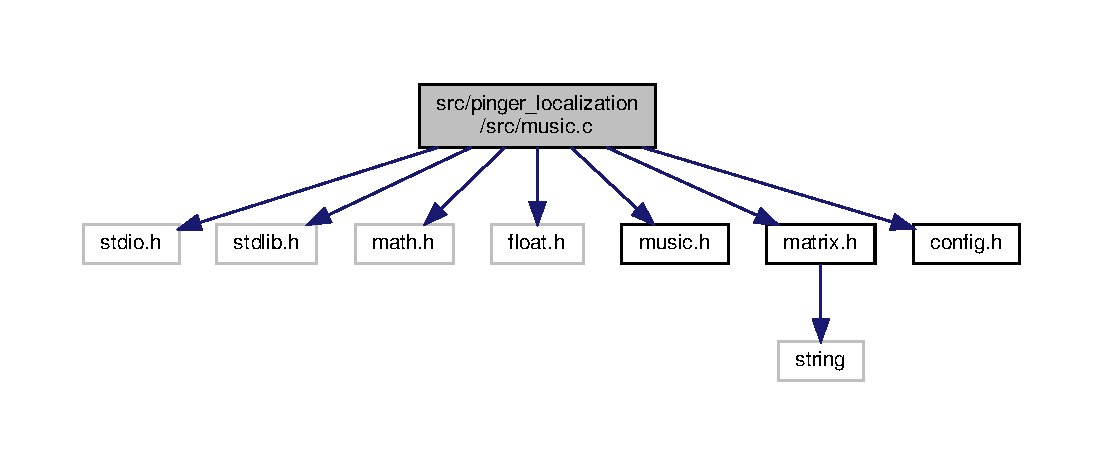
\includegraphics[width=350pt]{music_8c__incl}
\end{center}
\end{figure}
\subsection*{Functions}
\begin{DoxyCompactItemize}
\item 
void \hyperlink{music_8c_a046b73e9823c16ba6a3c7f5469d82cad}{dft} (double $\ast$ps)
\begin{DoxyCompactList}\small\item\em Computes a D\+FT at the pinger frequency for phase shifts. \end{DoxyCompactList}\item 
void \hyperlink{music_8c_a6aeb3e94a67f90f5a2cdd4f83a0ee7cb}{tdoa} (double $\ast$ps, double $\ast$tdoa)
\begin{DoxyCompactList}\small\item\em Computes the T\+D\+OA (time difference of arrival) between phase shifts. \end{DoxyCompactList}\item 
void \hyperlink{music_8c_ac7969308bd0fb9d760e3b38653439df2}{music} (double $\ast$\hyperlink{music_8h_a6aeb3e94a67f90f5a2cdd4f83a0ee7cb}{tdoa}, double $\ast$angle)
\begin{DoxyCompactList}\small\item\em Computes the D\+OA (direction of arrival) using T\+D\+O\+As. \end{DoxyCompactList}\end{DoxyCompactItemize}


\subsection{Detailed Description}
Functions used to compute D\+OA (direction-\/of-\/arrival) using M\+U\+S\+IC. 

\begin{DoxyAuthor}{Author}
David Zhang (Davarco) 
\end{DoxyAuthor}


\subsection{Function Documentation}
\mbox{\Hypertarget{music_8c_a046b73e9823c16ba6a3c7f5469d82cad}\label{music_8c_a046b73e9823c16ba6a3c7f5469d82cad}} 
\index{music.\+c@{music.\+c}!dft@{dft}}
\index{dft@{dft}!music.\+c@{music.\+c}}
\subsubsection{\texorpdfstring{dft()}{dft()}}
{\footnotesize\ttfamily void dft (\begin{DoxyParamCaption}\item[{double $\ast$}]{ps }\end{DoxyParamCaption})}



Computes a D\+FT at the pinger frequency for phase shifts. 


\begin{DoxyParams}{Parameters}
{\em ps} & The address where the M phase shifts (radians) will be written. \\
\hline
\end{DoxyParams}
\mbox{\Hypertarget{music_8c_ac7969308bd0fb9d760e3b38653439df2}\label{music_8c_ac7969308bd0fb9d760e3b38653439df2}} 
\index{music.\+c@{music.\+c}!music@{music}}
\index{music@{music}!music.\+c@{music.\+c}}
\subsubsection{\texorpdfstring{music()}{music()}}
{\footnotesize\ttfamily void music (\begin{DoxyParamCaption}\item[{double $\ast$}]{tdoa,  }\item[{double $\ast$}]{angle }\end{DoxyParamCaption})}



Computes the D\+OA (direction of arrival) using T\+D\+O\+As. 

M\+U\+S\+IC is limited to a \mbox{[}-\/90, 90\mbox{]} degree window. 0 is north, or X.


\begin{DoxyParams}{Parameters}
{\em tdoa} & The M T\+D\+O\+As (periods). \\
\hline
{\em angle} & The address where the D\+OA (degrees) will be written. \\
\hline
\end{DoxyParams}
\mbox{\Hypertarget{music_8c_a6aeb3e94a67f90f5a2cdd4f83a0ee7cb}\label{music_8c_a6aeb3e94a67f90f5a2cdd4f83a0ee7cb}} 
\index{music.\+c@{music.\+c}!tdoa@{tdoa}}
\index{tdoa@{tdoa}!music.\+c@{music.\+c}}
\subsubsection{\texorpdfstring{tdoa()}{tdoa()}}
{\footnotesize\ttfamily void tdoa (\begin{DoxyParamCaption}\item[{double $\ast$}]{ps,  }\item[{double $\ast$}]{tdoa }\end{DoxyParamCaption})}



Computes the T\+D\+OA (time difference of arrival) between phase shifts. 

The first T\+D\+OA value should be 0, as all the T\+D\+O\+As are calculated relative to the first phase shift.


\begin{DoxyParams}{Parameters}
{\em ps} & The M phase shifts (radians). \\
\hline
{\em tdoa} & The address where the M T\+D\+O\+As (periods) will be written. \\
\hline
\end{DoxyParams}

\hypertarget{music_8h}{}\section{src/pinger\+\_\+localization/src/music.h File Reference}
\label{music_8h}\index{src/pinger\+\_\+localization/src/music.\+h@{src/pinger\+\_\+localization/src/music.\+h}}


Function declarations for M\+U\+S\+IC (Multiple Signal Classification).  


This graph shows which files directly or indirectly include this file\+:\nopagebreak
\begin{figure}[H]
\begin{center}
\leavevmode
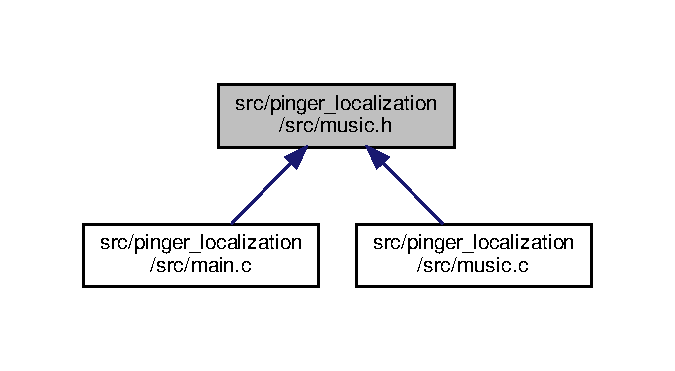
\includegraphics[width=324pt]{music_8h__dep__incl}
\end{center}
\end{figure}
\subsection*{Functions}
\begin{DoxyCompactItemize}
\item 
void \hyperlink{music_8h_a046b73e9823c16ba6a3c7f5469d82cad}{dft} (double $\ast$ps)
\begin{DoxyCompactList}\small\item\em Computes a D\+FT at the pinger frequency for phase shifts. \end{DoxyCompactList}\item 
void \hyperlink{music_8h_a6aeb3e94a67f90f5a2cdd4f83a0ee7cb}{tdoa} (double $\ast$ps, double $\ast$tdoa)
\begin{DoxyCompactList}\small\item\em Computes the T\+D\+OA (time difference of arrival) between phase shifts. \end{DoxyCompactList}\item 
void \hyperlink{music_8h_ac7969308bd0fb9d760e3b38653439df2}{music} (double $\ast$\hyperlink{music_8h_a6aeb3e94a67f90f5a2cdd4f83a0ee7cb}{tdoa}, double $\ast$angle)
\begin{DoxyCompactList}\small\item\em Computes the D\+OA (direction of arrival) using T\+D\+O\+As. \end{DoxyCompactList}\end{DoxyCompactItemize}


\subsection{Detailed Description}
Function declarations for M\+U\+S\+IC (Multiple Signal Classification). 

\begin{DoxyAuthor}{Author}
David Zhang (Davarco)  No known bugs. 
\end{DoxyAuthor}


\subsection{Function Documentation}
\mbox{\Hypertarget{music_8h_a046b73e9823c16ba6a3c7f5469d82cad}\label{music_8h_a046b73e9823c16ba6a3c7f5469d82cad}} 
\index{music.\+h@{music.\+h}!dft@{dft}}
\index{dft@{dft}!music.\+h@{music.\+h}}
\subsubsection{\texorpdfstring{dft()}{dft()}}
{\footnotesize\ttfamily void dft (\begin{DoxyParamCaption}\item[{double $\ast$}]{ps }\end{DoxyParamCaption})}



Computes a D\+FT at the pinger frequency for phase shifts. 


\begin{DoxyParams}{Parameters}
{\em ps} & The address where the M phase shifts (radians) will be written. \\
\hline
\end{DoxyParams}
\mbox{\Hypertarget{music_8h_ac7969308bd0fb9d760e3b38653439df2}\label{music_8h_ac7969308bd0fb9d760e3b38653439df2}} 
\index{music.\+h@{music.\+h}!music@{music}}
\index{music@{music}!music.\+h@{music.\+h}}
\subsubsection{\texorpdfstring{music()}{music()}}
{\footnotesize\ttfamily void music (\begin{DoxyParamCaption}\item[{double $\ast$}]{tdoa,  }\item[{double $\ast$}]{angle }\end{DoxyParamCaption})}



Computes the D\+OA (direction of arrival) using T\+D\+O\+As. 

M\+U\+S\+IC is limited to a \mbox{[}-\/90, 90\mbox{]} degree window. 0 is north, or X.


\begin{DoxyParams}{Parameters}
{\em tdoa} & The M T\+D\+O\+As (periods). \\
\hline
{\em angle} & The address where the D\+OA (degrees) will be written. \\
\hline
\end{DoxyParams}
\mbox{\Hypertarget{music_8h_a6aeb3e94a67f90f5a2cdd4f83a0ee7cb}\label{music_8h_a6aeb3e94a67f90f5a2cdd4f83a0ee7cb}} 
\index{music.\+h@{music.\+h}!tdoa@{tdoa}}
\index{tdoa@{tdoa}!music.\+h@{music.\+h}}
\subsubsection{\texorpdfstring{tdoa()}{tdoa()}}
{\footnotesize\ttfamily void tdoa (\begin{DoxyParamCaption}\item[{double $\ast$}]{ps,  }\item[{double $\ast$}]{tdoa }\end{DoxyParamCaption})}



Computes the T\+D\+OA (time difference of arrival) between phase shifts. 

The first T\+D\+OA value should be 0, as all the T\+D\+O\+As are calculated relative to the first phase shift.


\begin{DoxyParams}{Parameters}
{\em ps} & The M phase shifts (radians). \\
\hline
{\em tdoa} & The address where the M T\+D\+O\+As (periods) will be written. \\
\hline
\end{DoxyParams}

\hypertarget{simulate_8c}{}\section{src/pinger\+\_\+simulation/src/simulate.c File Reference}
\label{simulate_8c}\index{src/pinger\+\_\+simulation/src/simulate.\+c@{src/pinger\+\_\+simulation/src/simulate.\+c}}


Simulates sampling a pinger in an underwater environment.  


{\ttfamily \#include $<$stdio.\+h$>$}\newline
{\ttfamily \#include $<$stdlib.\+h$>$}\newline
{\ttfamily \#include $<$math.\+h$>$}\newline
{\ttfamily \#include \char`\"{}config.\+h\char`\"{}}\newline
Include dependency graph for simulate.\+c\+:
\nopagebreak
\begin{figure}[H]
\begin{center}
\leavevmode
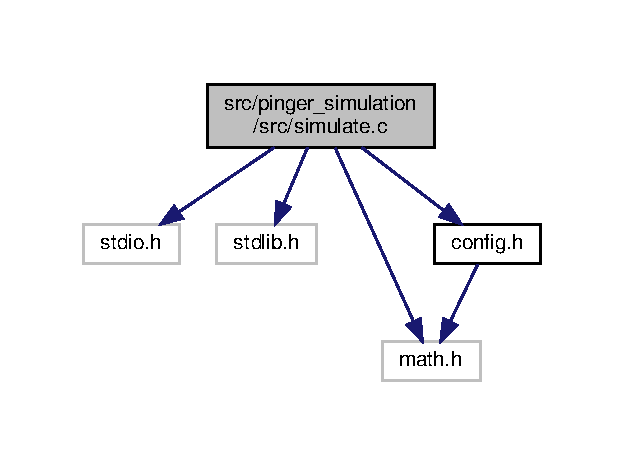
\includegraphics[width=300pt]{simulate_8c__incl}
\end{center}
\end{figure}
\subsection*{Functions}
\begin{DoxyCompactItemize}
\item 
\mbox{\Hypertarget{simulate_8c_ad1b4bb232d2a5d3362646c06a629f00d}\label{simulate_8c_ad1b4bb232d2a5d3362646c06a629f00d}} 
double {\bfseries randn} (double, double)
\item 
int \hyperlink{simulate_8c_ae66f6b31b5ad750f1fe042a706a4e3d4}{main} ()
\begin{DoxyCompactList}\small\item\em Simulator start. \end{DoxyCompactList}\end{DoxyCompactItemize}


\subsection{Detailed Description}
Simulates sampling a pinger in an underwater environment. 

\begin{DoxyAuthor}{Author}
David Zhang (davarco) 
\end{DoxyAuthor}
\begin{DoxyRefDesc}{Bug}
\item[\hyperlink{bug__bug000002}{Bug}]No known bugs. \end{DoxyRefDesc}


\subsection{Function Documentation}
\mbox{\Hypertarget{simulate_8c_ae66f6b31b5ad750f1fe042a706a4e3d4}\label{simulate_8c_ae66f6b31b5ad750f1fe042a706a4e3d4}} 
\index{simulate.\+c@{simulate.\+c}!main@{main}}
\index{main@{main}!simulate.\+c@{simulate.\+c}}
\subsubsection{\texorpdfstring{main()}{main()}}
{\footnotesize\ttfamily int main (\begin{DoxyParamCaption}{ }\end{DoxyParamCaption})}



Simulator start. 

This code simulates sampling a pinger by computing the theoretical phase shifts of each hydrophone, while adding noise to the measurements. It sends the data over a named pipe for the localization system to read.

\begin{DoxyReturn}{Returns}
Should not return. 
\end{DoxyReturn}

%--- End generated contents ---

% Index
\backmatter
\newpage
\phantomsection
\clearemptydoublepage
\addcontentsline{toc}{chapter}{Index}
\printindex

\end{document}
